\chapter{Nonlinear Endmember Extraction and Spectral Unmixing with Generative Simplex Mapping}\label{ch:robot-team-gsm}


In the previous chapter, we demonstrated how an unsupervised probabilistic model
like the GTM can be used to map the distribution of HSI spectra captured by the
UAV \textit{and} identify spectral signatures corresponding to unique sources in
the water. Unfortunately, the geometry of the GTM latent space does not
directly translate a mixture of sources and the coordinates in the latent space
are not directly interpretable. In this chapter, we introduce a new model for
non-linear endmember extraction and spectral unmixing of hyperspectral imagery
called Generative Simplex Mapping (GSM). The model represents endmember mixing
using a latent space with points sampled within a $(n-1)$-simplex corresponding
to the abundance of $n$ unique sources. Points in this latent space are
non-linearly mapped to reflectance spectra via a flexible function to account for
both linear and non-linear mixing effects. Due to the probabilistic formulation
of the GSM, spectral variability is also estimated by a precision parameter
describing the distribution of observed spectra. Model parameters are determined
using a generalized expectation-maximization algorithm which guarantees
non-negativity for endmember spectra. In the event of purely
linear mixing, non-linear contributions are naturally driven to zero.

The GSM outperforms three varieties of non-negative matrix factorization for both
endmember extraction accuracy and abundance estimation on a synthetic data set
of linearly mixed spectra from the USGS spectral library. In a second
experiment, the GSM is applied to real hyperspectral imagery captured over a
pond in North Texas. The model is able to accurately identify spectral
signatures corresponding to near-shore algae, water, and rhodmaine tracer dye
introduced into the pond to simulate water contamination by a localized
source. Abundance maps generated using the GSM accurately track evolution of
the dye plume as it mixes into the surrounding water.


\section{Motivation}


Many approaches have been developed to make sense of the HSI data. For example,
spectral indices such as the popular normalized difference vegetation index
(NDVI) can be computed by taking ratios of spectral bands tailored to track
specific reflectance characteristics
\cite{thenkabail-indices,thenkabail2018hyperspectral}. These indices have the
advantage of being easy to compute, but suffer from significant variability
between instruments while ignoring most of the information captured in HSI
spectra \cite{ndvi-variability}. An alternative approach is to pair HSI data
with in situ measurements to enable supervised models that map spectra directly
to parameters of interest. However, this approach relies on serendipitous
satellite overpasses above sensing sites to generate sufficient quantities of
aligned data for model training and evaluation. For example, Aurin et al.
combined data from over 30 years of oceanographic field campaigns with paired
satellite imagery to develop robust models for the inversion of key water
quality indicators such as colored dissolved organic matter
\cite{aurin2018remote}. This approach can be accelerated by combining UAV-based
hyperspectral imaging with rapid in situ data collection using autonomous boats
as demonstrated in Chapter~\ref{ch:robot-team-supervised}. However, these
supervised methods rely on \textit{a priori} knowledge of expected sources to
identify appropriate reference sensors for data collection. In light of these
limitations, unsupervised methods are needed that can expediently extract source
signatures from high-dimensional HSI.


The spatial resolution of hyperspectral imagers generally results in pixels with
mixed signals from multiple sources called endmembers. The task of unsupervised
source identification using HSI data therefore involves two steps: endmember
extraction and abundance estimation. Techniques such as vertex component
analysis (VCA), the pixel purity index (PPI), and N-FINDR solve this first task
by identifying HSI endmember spectra assuming the presence of some pure
(unmixed) pixels \cite{vca-orig, ppi-orig, N-FINDR-orig}. By further assuming a
linear mixing model (LMM) in which observed spectra are described by a linear
combination of endmembers with non-negative abundances, HSI can be unmixed using
a variety of techniques such as constrained least squares
\cite{spectral-unmixing-orig, fcls-unmixing}. Among these methods, Nonnegative
Matrix Factorization (NMF) is a widely used approach which extracts endmember
spectra and unmixes abundances simultaneously via matrix factorization
\cite{nmf-orig, unmixing-nmf-review, unmixing-nmf-review-2}. The update
equations for NMF can be formulated as multiplicative updates which guarantee
the non-negativity of endmember spectra and their associated abundances
\cite{nmf-algorithms}.  For this reason, the continued development of new NMF
varieties remains an active area of research.

In realistic scenes, multiple scattering and surface variability can easily
challenge the assumption of linear mixing as illustrated in
Figure~\ref{fig:multiple-scattering} \cite{heylen2014review}.
\begin{figure}[H]
  \centering
  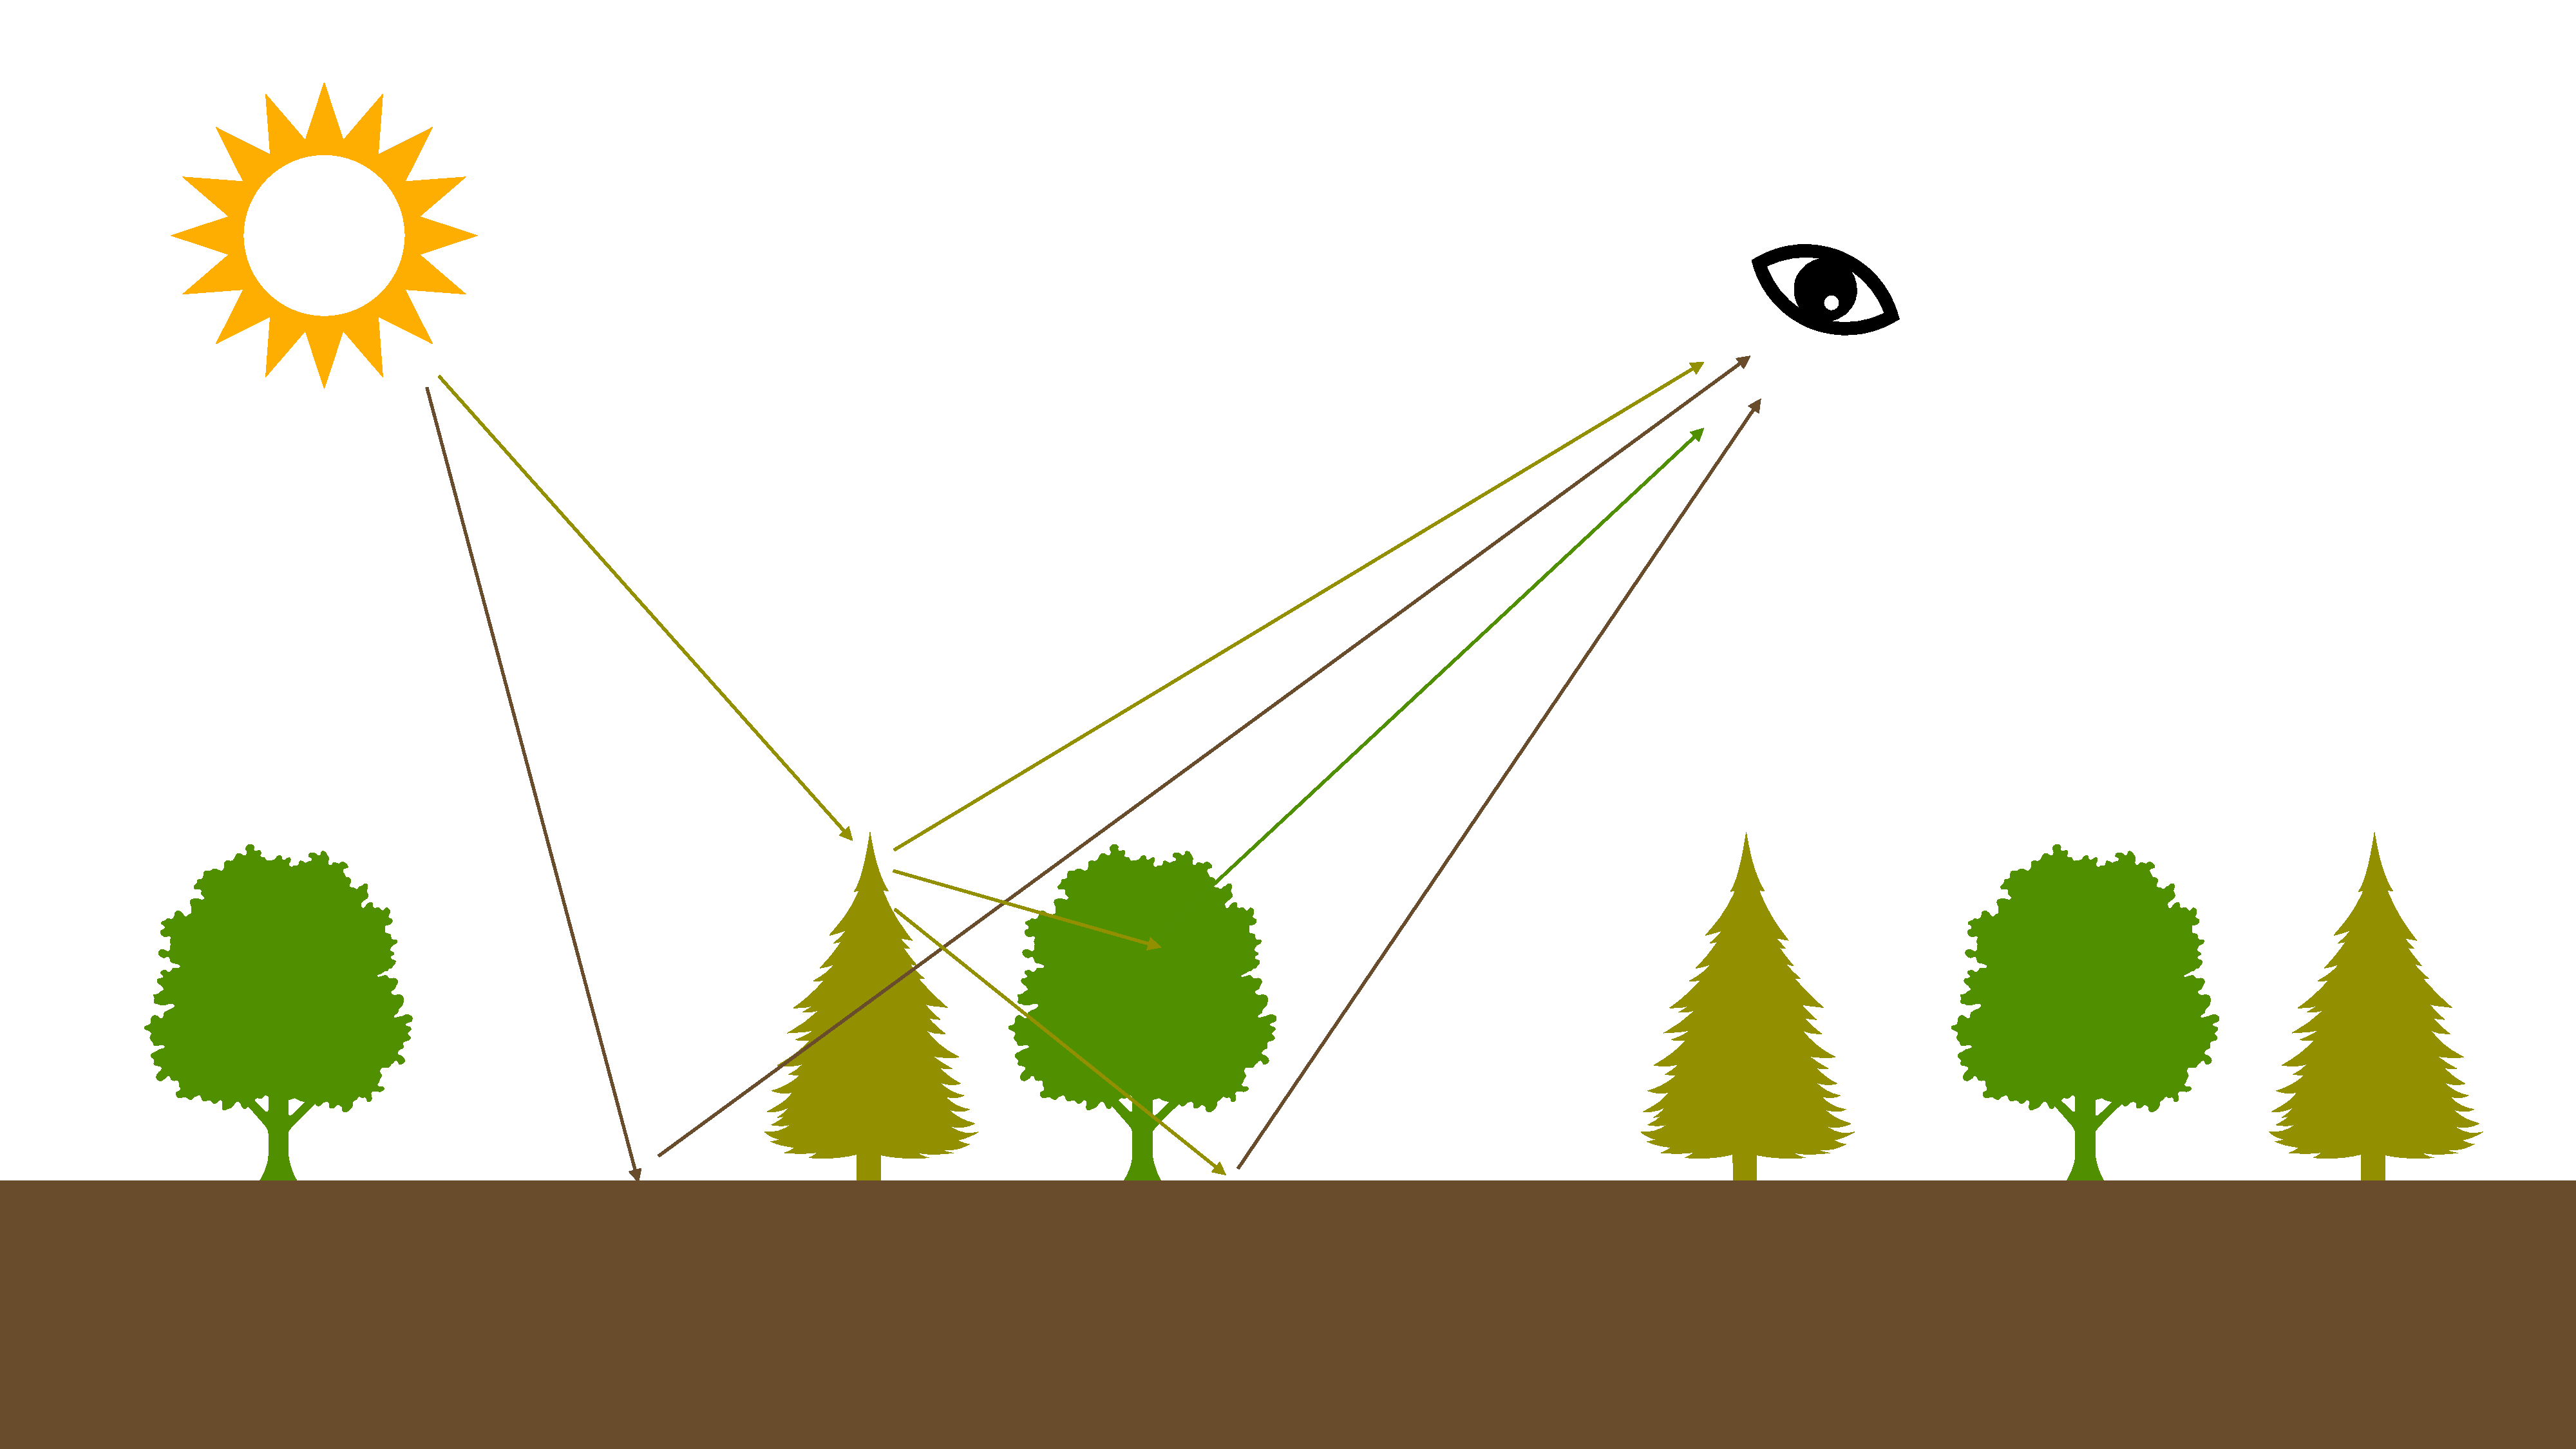
\includegraphics[width=0.7\columnwidth]{robot-team-gsm/multiple-scattering.pdf}
  \caption{Multiple Scattering: Light from the sun scatters off of individual
    surfaces such as tree leaves and the ground. Secondary
    scattering can occur when a scattered ray interacts with additional sources
    before being measured.}
  \label{fig:multiple-scattering}
\end{figure}
Water-based HSI specifically are prone to non-linear mixing effects due to absorption
features of dissolved and suspended substances, fluorescence of organic matter,
and particulate scattering in turbid waters \cite{hsi-absorption,
  hsi-fluorescence, hsi-turibidity}. With the growing popularity of deep
learning approaches in remote sensing, a variety of models based on autoencoder
architectures have been introduced for unmixing HSI data
\cite{non-negative-autoencoders,su2019daen,borsoi2019deep,palsson2020convolutional}.
However, the complexity introduced by these models significantly impacts
training time and decreases model interpretability. An ideal approach
should enable both endmember extraction and non-linear unmixing while accounting
for spectral variability.

The self-organizing map (SOM) presented in Chapter~\ref{ch:robot-team-gtm} is an
unsupervised machine learning method that
maps high-dimensional data to a low-dimensional grid while preserving the
topological relationships between data points \cite{kohonen-som-1}. This
low-dimensional representation provides a convenient way to visualize HSI data
while the weight vectors for each SOM node can be interpreted as representative
spectra \cite{cantero2004analysis, duran2007time,som-hsi}. If labelled reference
spectra are available, the SOM can be used to enable semi-supervised labeling of
HSI pixels \cite{riese2019supervised}. The SOM has also been shown to be
effective for the compression of HSIs acquired by a CubeSat
\cite{som-satellite}. Despite these capabilities, the SOM does not offer a
probabilistic interpretation and relies on a heuristic training procedure with
hyperparameters that can be challenging to tune. To address these shortcomings,
Bishop et al. introduced the Generative Topographic Mapping (GTM), a
probabilistic latent-variable model inspired by the SOM \cite{gtm-orig}. When
choosing a two-dimensional latent space, the GTM can be used to visualize the
distribution of HSI spectra while mapping the latent space nodes to the HSI data
space provides endmembers as demonstrated in Chapter~\ref{ch:robot-team-gtm}.
Unfortunately, the rectangular latent space grid employed by the GTM does not
directly translate into endmember
abundances. Additionally, the expectation-maximization (EM) algorithm used to
train the GTM does not guarantee non-negativity of GTM node spectra.

In this study, we introduce a new variant of the GTM dubbed Generative Simplex
Mapping (GSM), which can extract endmember spectra and unmix non-linear
mixtures. By replacing the rectangular latent space of the GTM with a gridded
$(n-1)$-simplex, the vertices of the GSM can be immediately interpreted as
endmembers corresponding to $n$ unique spectral signatures. The mapping from
the latent space to the HSI data space models signal mixing while barycentric
coordinates for the latent space simplex estimate relative endmember abundances.
Furthermore, by taking inspiration from the multiplicative updates of NMF, the
GSM algorithm maintains the non-negativity of resulting endmember spectra. If
only linear mixing is present, the GSM algorithm drives non-linear contributions
to $0$. Prior distributions included for GSM model weights yield hyperparameters
which can be tuned to control the smoothness of the resulting spectra and the
degree of non-linear mixing applied.

\section{Nonnegative Matrix Factorization}

In this section, we provide a brief overview of the non-negative matrix
factorization (NMF) method which will be compared against the GSM later in this
chapter. As a linear mixing model, NMF describes a dataset $\mathbf{X}$ by
\begin{equation}
  \mathbf{X} \approx \mathbf{W}\mathbf{H}
\end{equation}
where, for our purposes, $\mathbf{X}$ is a matrix of concatenated spectra, and
$\mathbf{W}$ and $\mathbf{H}$ are non-negative factor matrices. Fitting an NMF
model corresponds to solving for $\mathbf{W}$ and $\mathbf{H}$ which minimize
a cost function.

The most obvious choice for cost function is to use the squared residual error
corresponding to the Euclidean distance (i.e. Frobenius matrix norm):
\begin{equation}
  C = \lVert  \mathbf{X} - \mathbf{W}\mathbf{H} \rVert_F = \sum_m\sum_n \left( X_{mn} - \sum_k W_{mk}H_{kn} \right)^2.
\end{equation}

Differentiating with respect to $W_{ij}$, we find
\begin{align}
  \frac{\partial C}{\partial W_{ij}} &= \frac{\partial}{\partial W_{ij}}\sum_m\sum_n\left( X_{mn} - \sum_kW_{mk}H_{kn} \right)^2 \\
                                     &= \sum_m\sum_n 2\left( X_{mn} - \sum_k W_{mk}H_{kn} \right) \left( - H_{\lambda n}\delta_{mi}\delta_{\lambda j} \right)\\
                                     &= \sum_n\sum_k -2X_{in}H_{jn} + W_{ik}H_{kn}H_{jn}
\end{align}
which leads to the matrix equation
\begin{equation}
  \frac{\partial C}{\partial \mathbf{W}} = -2\mathbf{X}\mathbf{H}^T + 2\mathbf{W}\mathbf{H}\mathbf{H}^T.
\end{equation}

Repeating the process for $\mathbf{H}$, we obtain
\begin{equation}
  \frac{\partial C}{\partial \mathbf{H}} = -2\mathbf{W}^T\mathbf{X} + 2\mathbf{W}^T\mathbf{W}\mathbf{H}.
\end{equation}

A standard optimization approach would then be to perform block-gradient descent
for $\mathbf{W}$ and $\mathbf{H}$ whereby
\begin{equation}
  \begin{cases}
    \mathbf{W}^{\text{next}} = \mathbf{W} - \eta_{W}\frac{\partial C}{\partial \mathbf{W}} \\
    \mathbf{H}^{\text{next}} = \mathbf{H} - \eta_{H}\frac{\partial C}{\partial \mathbf{H}}
  \end{cases}
\end{equation}
for learning rates $\eta_{W}$ and $\eta_{H}$. However clearly the subtraction in
these update equations could result in negative entries in $\mathbf{W}$ and
$\mathbf{H}$. To address this, \cite{nmf-orig} allow $\eta_{W}$ and $\eta_{H}$
to be \textit{matrix valued} corresponding to adaptive learning rates for each
matrix element. Then, they chose their values result in multiplicative updates
which guarantee non-negativity of $\mathbf{W}$ and $\mathbf{H}$. The result is
\begin{equation}
  \begin{cases}
    W^{\text{new}}_{ik} = W_{ik} \cdot    \dfrac{(\mathbf{X}\mathbf{H}^T)_{ik}}{(\mathbf{W}\mathbf{H}\mathbf{H}^T)_{ik}} \\
    H^{\text{new}}_{kj} = H_{kj} \cdot \dfrac{(\mathbf{W}^T\mathbf{X})_{kj}}{(\mathbf{W}^T\mathbf{W}\mathbf{H})_{kj}}
  \end{cases}
\end{equation}
which are computed element-wise.

Other cost functions can be used in the formulation of the NMF model. In this
study, we consider two additional versions: a generalized KL-divergence cost
function, and an $\ell_{2,1}$-norm based cost function. The corresponding cost
functions are given by
\begin{align}
  C_{KL} &= \sum_m\sum_n\left( X_{mn}\ln\frac{X_{mn}}{\sum_kW_{mk}H_{kn}} - X_{mn} + \sum_kW_{mk}H_{kn} \right) \\
  C_{2,1} &= \sum_n\left( \sum_m \left( X_{mn} - \sum_k W_{mk}H_{kn} \right)^2 \right)^{1/2}.
\end{align}
The KL-divergence update equations take the form
\begin{equation}
  \begin{cases}
    W^{\text{next}}_{ik} = W_{ik} \cdot \dfrac{\sum_s X_{is}H_{ks}/(\mathbf{W}\mathbf{H})_{is}}{\sum_s H_{ks}} \\
    H^{\text{next}}_{kj} = H_{kj} \cdot \dfrac{\sum_s W_{sk}X_{sj}/(\mathbf{W}\mathbf{H})_{sj}}{\sum_sW_{sj}}
  \end{cases}
\end{equation}
while the $\ell_{2,1}$ update equations are
\begin{equation}
  \begin{cases}
    W^{\text{new}}_{ik} = W_{ik} \cdot \dfrac{(\mathbf{X}\mathbf{D}\mathbf{H}^T)_{ik}}{(\mathbf{W}\mathbf{H}\mathbf{D}\mathbf{H}^T)_{ik}} \\
    H^{\text{new}}_{kj} = H_{kj} \cdot \dfrac{(\mathbf{W}^T\mathbf{X}\mathbf{D})_{kj}}{(\mathbf{W}^T\mathbf{W}\mathbf{H}\mathbf{D})_{kj}}
  \end{cases}
\end{equation}
An open-source implementation of these three algorithms was developed for this study and is
accessible at
(\url{https://github.com/john-waczak/MLJNonnegativeMatrixFactorization.jl}, last
accessed 2024-09-16).

\section{GSM}

In the original GTM formulation, the data vectors $\mathbf{x}$ (reflectance spectra) are
described by latent variables $\xi$ mapped into the data space by a non-linear
function $\psi$. The data space distribution is taken to be normal with the
precision parameter $\beta$ to account for measurement noise and spectral
variability. The GSM uses same structure, that is
\begin{equation}\label{eqn:data-space-distribution}
    p(\mathbf{x} \mid \mathbf{z}, \mathbf{W}, \beta) = \left(\frac{\beta}{2\pi} \right)^{D/2}\exp\left( -\frac{\beta}{2}\lVert \psi(\mathbf{z}; \mathbf{W}) - \mathbf{x} \rVert^2 \right)
\end{equation}
where we have used $\mathbf{z}$ to represent the latent variables of the GSM, and
$\mathbf{W}$ are model weights which parameterize the mapping $\psi$.

Assuming data are uniformly sampled from an embedded manifold in the data space,
the GTM models the latent space using a rectangular grid with $K$-many nodes of
equal prior probability. To adapt the GTM to describe endmember mixing, the GSM
makes two key changes. The first is to replace the rectangular GTM grid with a
gridded simplex with $N_v$ vertices. The barycentric coordinates for each node
then describe the relative abundance of each endmember with each vertex
corresponding to a pure endmember. The second change is to replace equal prior
probabilities with adaptive mixing coefficients $\pi_k$ to allow the GSM to
model HSI with nonuniform mixing distributions. Together, this leads to a latent
space prior distribution given by
\begin{equation}\label{eqn:latent-distribution}
    p(\mathbf{z}) = \sum\limits_k^K \pi_k \, \delta(\mathbf{z} - \mathbf{z}_k) \quad\text{where}\quad  \sum_k^K\pi_k = 1.
\end{equation}

For a data set containing $N$-many records, these definitions yield a log
likelihood function given by
\begin{equation}\label{eqn:llh}
    \mathscr{L} = \sum\limits_n^N \ln \left( \sum\limits_k^K \pi_k \, p(\mathbf{x}_n \mid \mathbf{z}_k, \mathbf{W}, \beta) \right)
\end{equation}
which can be maximized to obtain optimal values for model weights $\mathbf{W}$,
mixing coefficients $\pi_k$, and precision $\beta$. Rather than optimizing
Eq~\ref{eqn:llh} directly, we instead choose a particular form for $\psi$ to
allow fitting the GSM via an EM algorithm.

In the standard LMM model, the mapping $\psi$ is given by
$\psi(\mathbf{z};\mathbf{W}) = \mathbf{W}\mathbf{z}$ where the columns
of $\mathbf{W}$ correspond to endmember spectra. To model non-linear mixing, $\mathbf{z}$
is replaced by the output of $M$-many activation functions such that $\psi(\mathbf{z};\mathbf{W})
= \mathbf{W}\phi(\mathbf{z})$. The activations applied to each GSM node can then be
collected to form a matrix with elements $\Phi_{km} = \phi_m(\mathbf{z}_k)$. For $m \leq
N_v$, we take $\Phi_{km} = [\mathbf{z_{k}}]_m$ (the $m$-th coordinate of the $k$-th node) to
model linear mixing. The remaining  $M-N_v$ activations are computed using
radial basis functions (RBF) with centers $\mu_m$
distributed throughout the simplex (but not at the vertices) with
\begin{equation}\label{eq:act-function}
    \Phi_{km} = \begin{cases}
        \dfrac{s - \lVert \mathbf{z}_k - \mu_m \rVert}{s}; & \lVert z_k - \mu_m \rVert \leq s \\
        0; & \lVert z_k - \mu_m \rVert > s
    \end{cases}
\end{equation}
where $s$ is the spacing between RBF centers. In this form, the first $N_v$
columns of $\mathbf{W}$ correspond to endmember spectra, while the remaining
columns account for additional non-linear effects. For linear mixing, the GSM
training algorithm should therefore drive $W_{dm}$ to $0$ for $m\geq N_v$. A
visualization of the GSM model is shown in Figure~\ref{fig:gsm-diagram}.


\begin{figure}[H]
  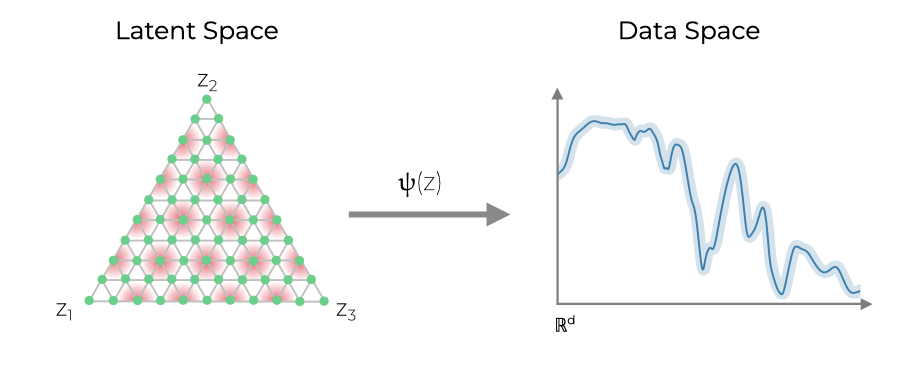
\includegraphics[width=\columnwidth]{robot-team-gsm/methods/gsm/gsm-diagram.png}
  \caption{Illustration of the GSM. The latent space consists of a grid of
    $K$-many points (green dots) distributed throughout a simplex with $N_v$
    vertices. Barycentric coordinates of each node in the simplex correspond to
    the relative abundance of $N_v$-many unique sources. Here, $N_v=3$ has been
    chosen for illustrative purposes. Nodes are mapped into the data space via
    the map $\psi(z)$ utilizing $M$-many radially symmetric basis functions
    (red). Spectral variability is estimated via the precision parameter $\beta$
    shown here in the data space as a light blue band around the spectrum given
    by $\psi(z)$.}
  \label{fig:gsm-diagram}
\end{figure}

To further constrain the model, we introduce prior distributions on the weights
$\mathbf{W}$. For $m\leq N_v$ we take $W_{dm}\sim\mathcal{N}(0, \lambda_e^{-1})$
corresponding to a zero-mean Gaussian with variance $\lambda_e^{-1}$. For
$m>N_v$ we use a zero-mean Laplace distribution,
$W_{dm}\sim\dfrac{\lambda_w}{2}\exp(-\lambda_w\lvert W_{dm}\rvert)$, with scale
parameter $\lambda_w^{-1}$. Under these choices $\lambda_e$ corresponds to $L_2$
regularization on endmember spectra while $\lambda_w$ corresponds to $L_1$
regularization on the non-linear activations. In other words, $\lambda_e$
governs the smoothness of the resulting endmembers while $\lambda_w$ encourages
sparsity for the non-linear contributions.


An EM algorithm for the GSM model can now be formulated as follows. Suppose that
we have current estimates for the model weights $\mathbf{W}$, mixing
coefficients $\pi_k$, and precision parameter $\beta$. During the expectation
step we compute the posterior probabilities, that is, the responsibility of each
GSM node for each spectrum in the data set:
\begin{equation}\label{eq:responsibility}
    R_{kn}  = p(\mathbf{z}_k \mid \mathbf{x}_n, \mathbf{W}, \beta) = \dfrac{\pi_k \, p(\mathbf{x}_n \mid \mathbf{z}_k, \mathbf{W}, \beta)}{\sum\limits_{k'}^K \pi_{k'} \, p(\mathbf{x}_n \mid \mathbf{z}_{k'}, \mathbf{W}, \beta)}.
\end{equation}
For the maximization step, we consider the expectation of the penalized
complete data log-likelihood given by
\begin{equation}\label{eq:complete-data-llh}
\begin{aligned}
    Q &= \sum_n^N\sum_k^K R_{kn} \left(\ln\pi_k + \frac{D}{2}\ln\left(\frac{\beta}{2\pi}\right) - \frac{\beta}{2}\sum_d^D\left(\sum_m^M W_{dm}\Phi_{km} - X_{nd}\right)^2\right) \\
    &\qquad + \frac{N_vD}{2}\ln\left(\frac{\lambda_e}{2\pi}\right) - \frac{\lambda}{2}\sum_d^D \sum_{m=1}^{N_v} W_{dm}^2  \\
    &\qquad + (M-N_v)D\ln\left(\dfrac{\lambda_w}{2}\right) - \lambda_w\sum_d^D\sum_{m=N_v+1}^{M} W_{dm}
\end{aligned}
\end{equation}
where $X_{nd}$ is the $d$-th component of the $n$-th spectrum in the data set.
Eq~\ref{eq:complete-data-llh} is then maximized with respect to $\pi_k$,
$\beta$, and $\mathbf{W}$ to obtain new parameter values.

For $\pi_k$, optimization can be performed using Lagrange multipliers to
maintain the condition that $\sum_k\pi_k=1$. Doing so yields
\begin{equation}\label{eq:pi-update}
    \pi_k^{\text{new}}  = \frac{1}{N}\sum_n R_{kn}.
\end{equation}

Optimization of Eq~\ref{eq:complete-data-llh} with respect to $\mathbf{W}$ leads
to a linear system which can be solved using standard numerical methods.
However, in this form, we cannot guarantee the non-negativity of $\mathbf{W}$
required to describe reflectance spectra. Therefore, we take inspiration from
the multiplicative updates for NMF introduced by Lee and Seung \cite{nmf-orig}.
A standard gradient-based update for $\mathbf{W}$ would normally take the form
\begin{equation}
    \mathbf{W}_{\text{new}} = \mathbf{W} + \eta\frac{\partial Q}{\partial \mathbf{W}}
\end{equation}
for some learning rate $\eta$. Therefore, we differentiate (see
Appendix~\ref{appendix:gsm-deriv}) to obtain
\begin{equation}
    \frac{\partial Q}{\partial \mathbf{W}} = -\beta \mathbf{W}\mathbf{\Phi}^T\mathbf{G}\mathbf{\Phi} - \mathbf{\Lambda} + \beta \mathbf{X}^T\mathbf{R}^T\mathbf{\Phi}
\end{equation}
where $\mathbf{G}$ is a diagonal matrix with $G_{kk} = \sum_n R_{kn}$ and
$\mathbf{\Lambda}$ is given by
\begin{equation}
    \Lambda_{dm} = \begin{cases}
        \lambda_e W_{dm}, & m \leq N_v \\
        \lambda_w, & m > N_v
    \end{cases}
\end{equation}
If we allow individual learning rates $\eta_{dm}$ for each element of
$\mathbf{W}$, then choosing
\begin{equation}
    \eta_{dm} = \frac{W_{dm}}{\left(\beta \mathbf{W}\mathbf{\Phi}^T\mathbf{G}\mathbf{\Phi}\right)_{dm} + \Lambda_{dm}}
\end{equation}
results in a multiplicative update rule given by
\begin{equation}\label{eq:W-update}
    W_{dm}^{new}  = W_{dm} \cdot \dfrac{\left(\beta \mathbf{X}^T\mathbf{R}^T\mathbf{\Phi}\right)_{dm}}{\left(\beta \mathbf{W}\mathbf{\Phi}^T\mathbf{G}\mathbf{\Phi}\right)_{dm} + \Lambda_{dm}}
\end{equation}
From Eq~\ref{eq:W-update}, it is clear that we are multiplying $W_{dm}$ by
strictly non-negative values, and therefore, non-negative $W_{dm}$ will remain
so during each update. This update can also be repeated multiple times during
each M-step to accelerate convergence.

Optimizing Eq~\ref{eq:complete-data-llh} with respect to $\beta$ yields the final update equation:
\begin{equation}\label{eq:beta-update}
    \frac{1}{\beta^{\text{new}}}  = \frac{1}{ND}\sum\limits_n^N\sum\limits_k^K R_{kn}\lVert \psi(\mathbf{z}_k; \mathbf{W}) - x_n \rVert^2.
\end{equation}

To train a GSM model, weights $\mathbf{W}$ are randomly initialized to positive
values. The mixing coefficients are initially set to $\pi_k = 1/K$. Finally, the
precision parameter $\beta$ is initialized to the variance of the $(N_v+1)$-th
principal component. After initialization, the expectation and maximization
steps are repeated in turn until $Q$ converges to a predetermined tolerance
level. For large $N_v$ we note that generating a regular grid within the simplex
becomes cumbersome as the number of grid nodes scales as ${k + N_v - 2 \choose
  N_v - 1}$ for $k$ nodes per edge. An alternative approach is to randomly
sample points within the simplex to obtain a total of $K$ nodes. A Dirichlet
distribution
\begin{equation}
    p(\mathbf{z}) = \frac{\Gamma(\sum_i^{N_v}\alpha_i)}{\prod_{i}^{N_v}\Gamma(\alpha_i)} \prod_{i}^{N_v} [\mathbf{z}]_i^{\alpha_i-1}
\end{equation}
with all $\alpha_i=1$ can be used to uniformly sample within the simplex. Since
the mixing coefficients $\pi_k$ are adaptive, variability in node separation
should not significantly impact the resulting GSM.

The probabilistic form of the GSM means that a variety of information criteria
can be used to evaluate the model fits. In this study we consider two metrics,
the Bayesian Information Criterion (BIC),
\begin{equation}
   \text{BIC} = P\ln(N) - 2\mathscr{L},
\end{equation}
and the Akaike Information Criterion (AIC),
\begin{equation}
    \text{AIC} = 2P - 2\mathscr{L}
\end{equation}
where $P$ is the total number of model parameters and $\mathscr{L}$ is the log
likelihood from Eq~\ref{eqn:llh}.

The map $\psi$ provides the representation of each node $z_k$ in the data space.
Importantly, applying $\psi$ to each vertex extracts endmember spectra from the
GSM. Slices $R_{\left[:,n\right]}$ of the matrix $\mathbf{R}$ define the
responsibility of each latent node $\mathbf{z}_k$ for the $n$-th spectrum
$\mathbf{x}_n$ in the data set. Therefore once the GSM has been trained,
$\mathbf{R}$ can be used to unmix endmember abundances by representing each
record in the latent space via the mean:
\begin{equation}
    \hat{\mathbf{z}}_n = \sum_k^K R_{kn}\mathbf{z}_k.
\end{equation}

A freely available implementation of the GSM is provided at \cite{gtm-code}. The
code is written in the Julia programming language and follows the Machine
Learning in Julia (MLJ) common interface \cite{bezanson2012julia, blaom2020mlj}.


\section{Study Overview}

\subsection{Linear Mixing: Comparison to NMF}\label{sec:experiments}

To illustrate the effectiveness of the GSM, we first demonstrate its ability to
model simple linear mixing by driving non-linear weights to zero during the
fitting process. To this end, a synthetic data set comprising linear mixtures of
three sample spectra from the U.S. Geological Survey digital spectral library
\cite{usgs-spectra} was generated by sampling $1000$ abundance vectors from a
Dirichlet distribution with $\alpha_1=\alpha_2=\alpha_3=1/3$. These source
spectra and abundances are visualized in Figure~\ref{fig:usgs-data}.

\begin{figure}[H]
  \centering
  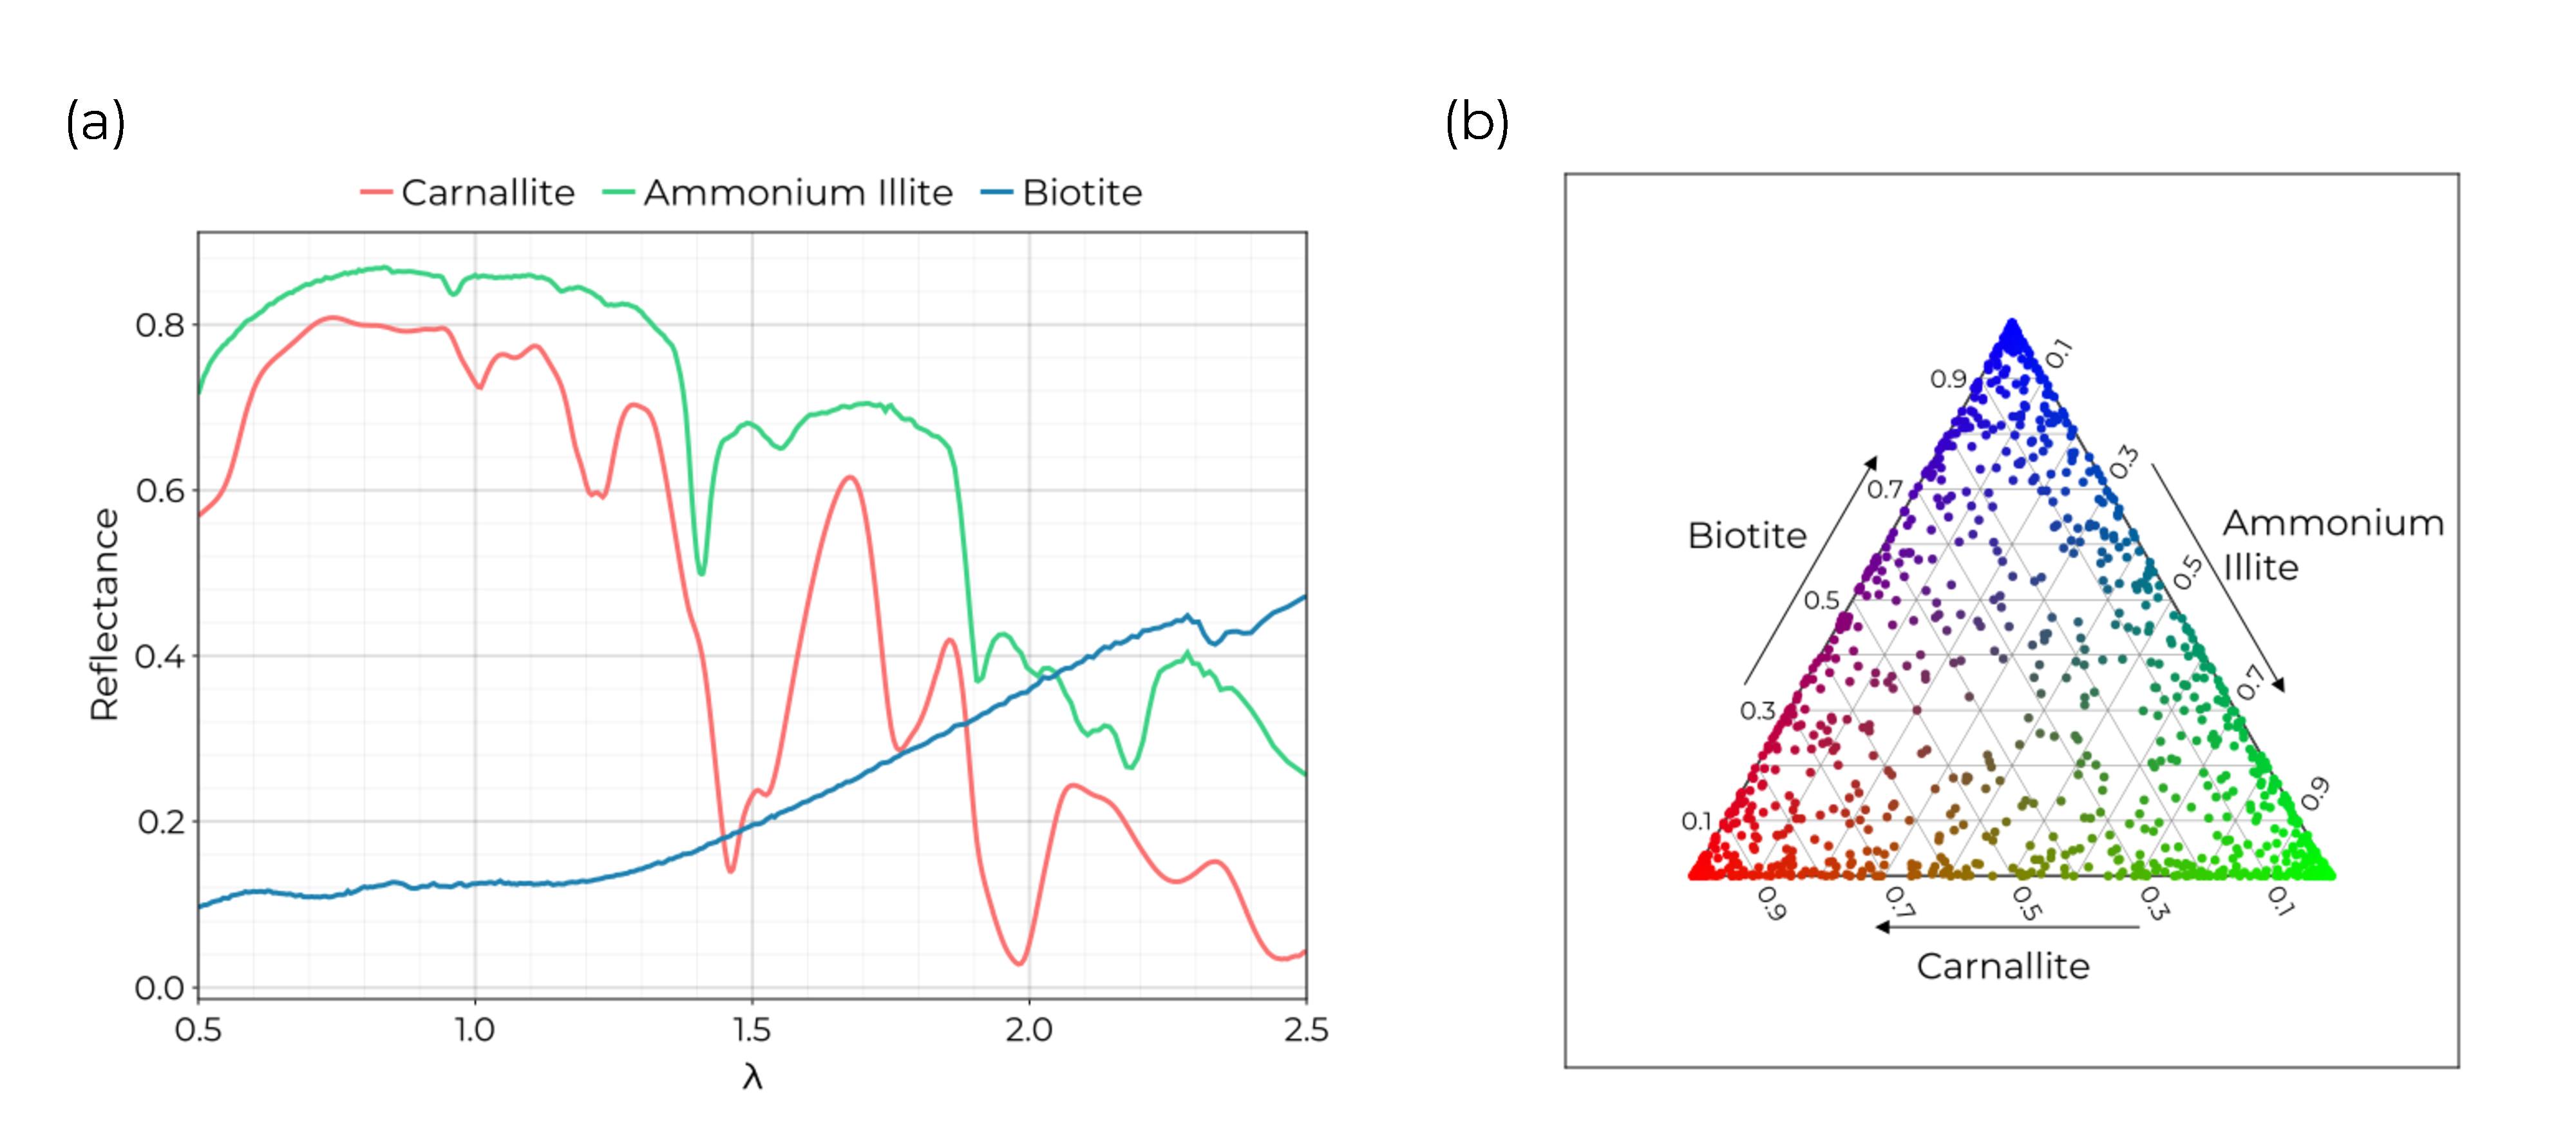
\includegraphics[width=\columnwidth]{robot-team-gsm/methods/usgs/usgs-dataset.pdf}
  \caption{Synthetic data set formed from USGS spectra. \textbf{(a)} Spectra
    from the USGS spectral database used as the ground truth endmembers. These
    spectra were selected following the example in ref. \cite{vca-orig}.
    \textbf{(b)} The abundance distribution sampled for in the data set. Samples
    were generated from a Dirichlet distribution with
    $\alpha_1=\alpha_2=\alpha_3=1/3$.}
  \label{fig:usgs-data}
\end{figure}

Zero-mean Gaussian noise was added to the data to yield $9$ data sets with
signal-to-noise ratios (SNR) ranging from $0$ to $\infty$ to examine the impact
of random noise on GSM performance. For each of these data sets, a GSM was
trained using $25$ nodes per edge with $\lambda_e$ set to the default value of
$0.01$ and $\lambda_w$ fixed to $100$. The large value of $\lambda_w$ was chosen
to encourage the GSM to prefer models with limited non-linear mixing.


For comparison, NMF models were also trained on each data set as this method is
both highly popular and does not include the pure-pixel assumption common to
other technqieus like VCA and PPI. Countless variations on the original NMF
method have been introduced into the literature with one review identifying more
than $100$ distinct NMF variations \cite{unmixing-nmf-review}. For the purpose
of evaluating the GSM, we considered the standard $\ell_2$ and KL-divergence
formulations introduced by Lee and Seung \cite{nmf-algorithms}. We also included
the robust $\ell_{2,1}$ NMF as described by Kong et al \cite{nmf-l21}.


Four metrics were used to compare model performance. For endmember extraction
the mean spectral angle and mean RMSE between true endmembers $\rho_i$ and
extracted endmembers $\hat{\rho}_i$ were computed where the spectral angle for
the $i$-th endmember is defined as
\begin{equation}
    \theta(\rho_i, \hat{\rho}_i) =  \arccos\left( \dfrac{\langle \rho_i, \hat{\rho}_i \rangle}{\lVert \rho_i \rVert \cdot \lVert \hat{\rho}_i \rVert}\right)
\end{equation}
and the RMSE for the $i$-th endmember is
\begin{equation}
    \text{RMSE}(\rho_i, \hat{\rho}_i) = \sqrt{\frac{1}{D-1}\sum_d^D\left(\rho_i(\lambda_d) - \hat{\rho}_i(\lambda_d) \right)^2}.
\end{equation}
Abundance estimation was similarly evaluated using the Mean RMSE between true
abundance and estimated abundance values for each endmember. Finally, the
reconstruction RMSE, that is, the RMSE computed between the original data set
and the data set reconstructed via the extracted endmembers and their associated
abundances was computed. This provides a model-agnostic criterion to guarantee
that each model sufficiently converged during training.

\subsection{Non-linear Mixing: Water Contaminant Identification}\label{sec:real-experiments}

To assess the ability of the GSM to unmix realistic scenes likely to involve
non-linear mixing effects, we consider a data set of real HSI collected in
Montague, North Texas on 9 December 2020 using the robot team described in
Chapter~\ref{ch:robot-team}. Rhodamine dye, a commonly used tracer in
hydrological studies, was released into a pond to simulate a potential
contaminant source. Two UAV flights spaced 15 minutes apart were used to capture
the evolution of the plume as it dispersed into the surrounding water.

The UAV flights were performed near solar noon to maximize the amount of
sunlight illuminating the water. For this pond in North Texas, this corresponded
to an average solar zenith angle of $56.7^{\circ}$ resulting in HSI with
negligible sunglint effects.

From the collected HSI, a water-only pixel mask was generated by identifying all
pixel spectra with a normalized difference water index (NDWI) greater than
$0.25$ as defined in ref. \cite{ndwi}. Of these water pixels, a combined data
set of $15,000$ spectra was sampled for GSM training. As a final processing
step, reflectance spectra were limited to $\lambda \leq 900$ nm as wavelengths
above this threshold showed significant noise.

In order to justify values for the appropriate number of endmembers, the final
data set was decomposed using principal component analysis (PCA). A plot of the
explained variance organized by PCA component is shown in
Figure~\ref{fig:robot-team-pca}

\begin{figure}[!h]
  \centering
  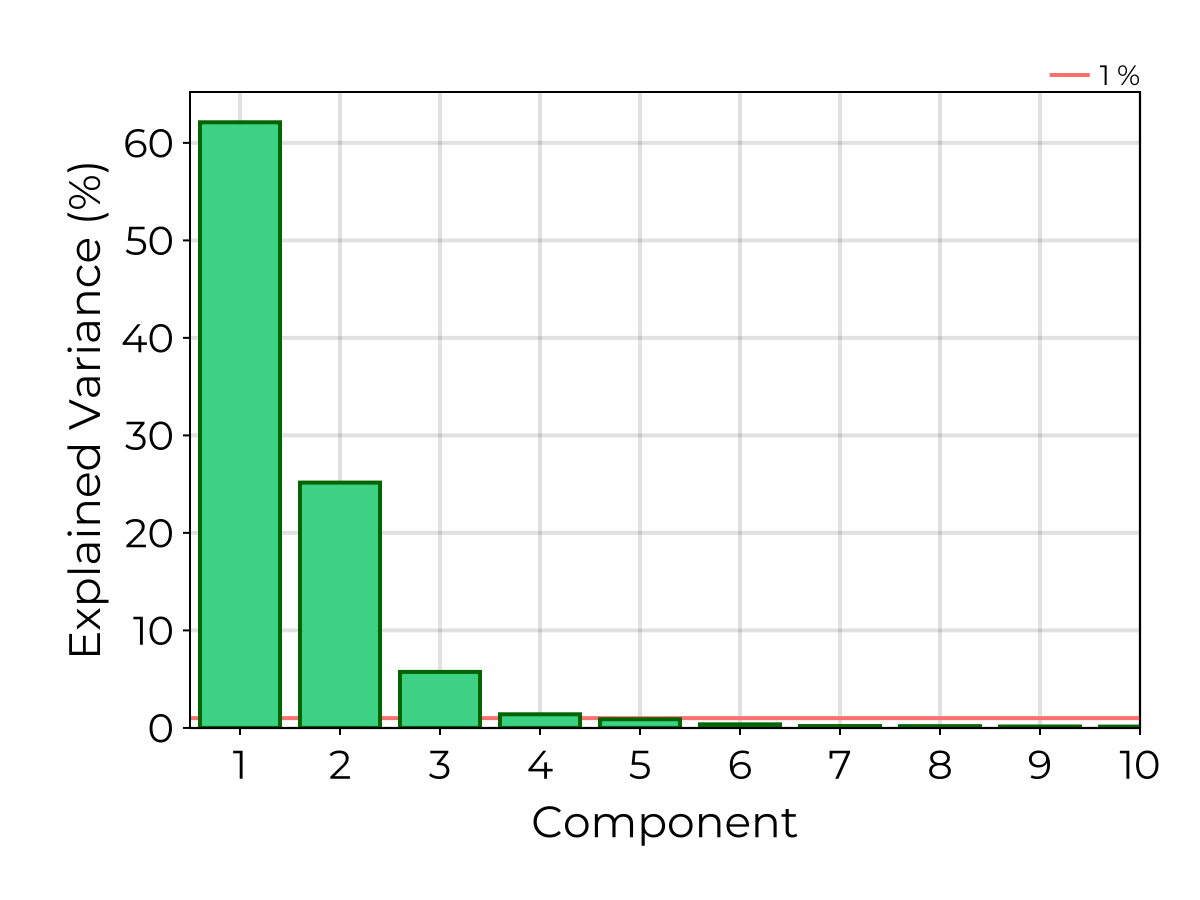
\includegraphics[width=0.60\columnwidth]{robot-team-gsm/results/robot-team/pca-variance.png}
  \caption{Explained variance of PCA components for the real HSI data set. A red
    horizontal line is superimposed on the graph, marking an explained variance
    of $1\%$. All components past the fourth explain less than $1\%$ of the
    observed variance.}
  \label{fig:robot-team-pca}
\end{figure}

The PCA decomposition of the data suggests that at least $3$ endmembers should
be used for a mixing model and beyond $6$ there is little added benefit. Based
on these observations, multiple GSM models were trained with $N_v$ ranging from
$3$ to $6$, $\lambda_e$ ranging from $0.001$ to $1.0$, and $\lambda_w$ ranging
from $1$ to $1000$ in order to explore the GSM parameter space. From these, a
final model was identified using the BIC, AIC, and reconstruction RMSE. The
resulting GSM was then explored to examine extracted endmembers and map the
evolution of the rhodamaine plume by using the abundances given by the latent
space representation of each pixel in the HSI.



\section{Results}


\subsection{Linear Mixing}

The results of GSM training on the synthetic linear mixing data set described in
Sec~\ref{sec:experiments} are illustrated in Figure~\ref{fig:usgs-fits}. Three
versions of NMF were trained corresponding to Euclidean ($\ell_2$),
KL-Divergence, and $\ell_{2,1}$ cost functions. GSM models using both a regular
simplex grid and a grid of points sampled using a uniform Dirichlet distribution
(referred to as a \textit{big} GSM model) were trained to compare performance in
linear mixing tasks.

\newpage

\begin{figure}[H]
  \centering
  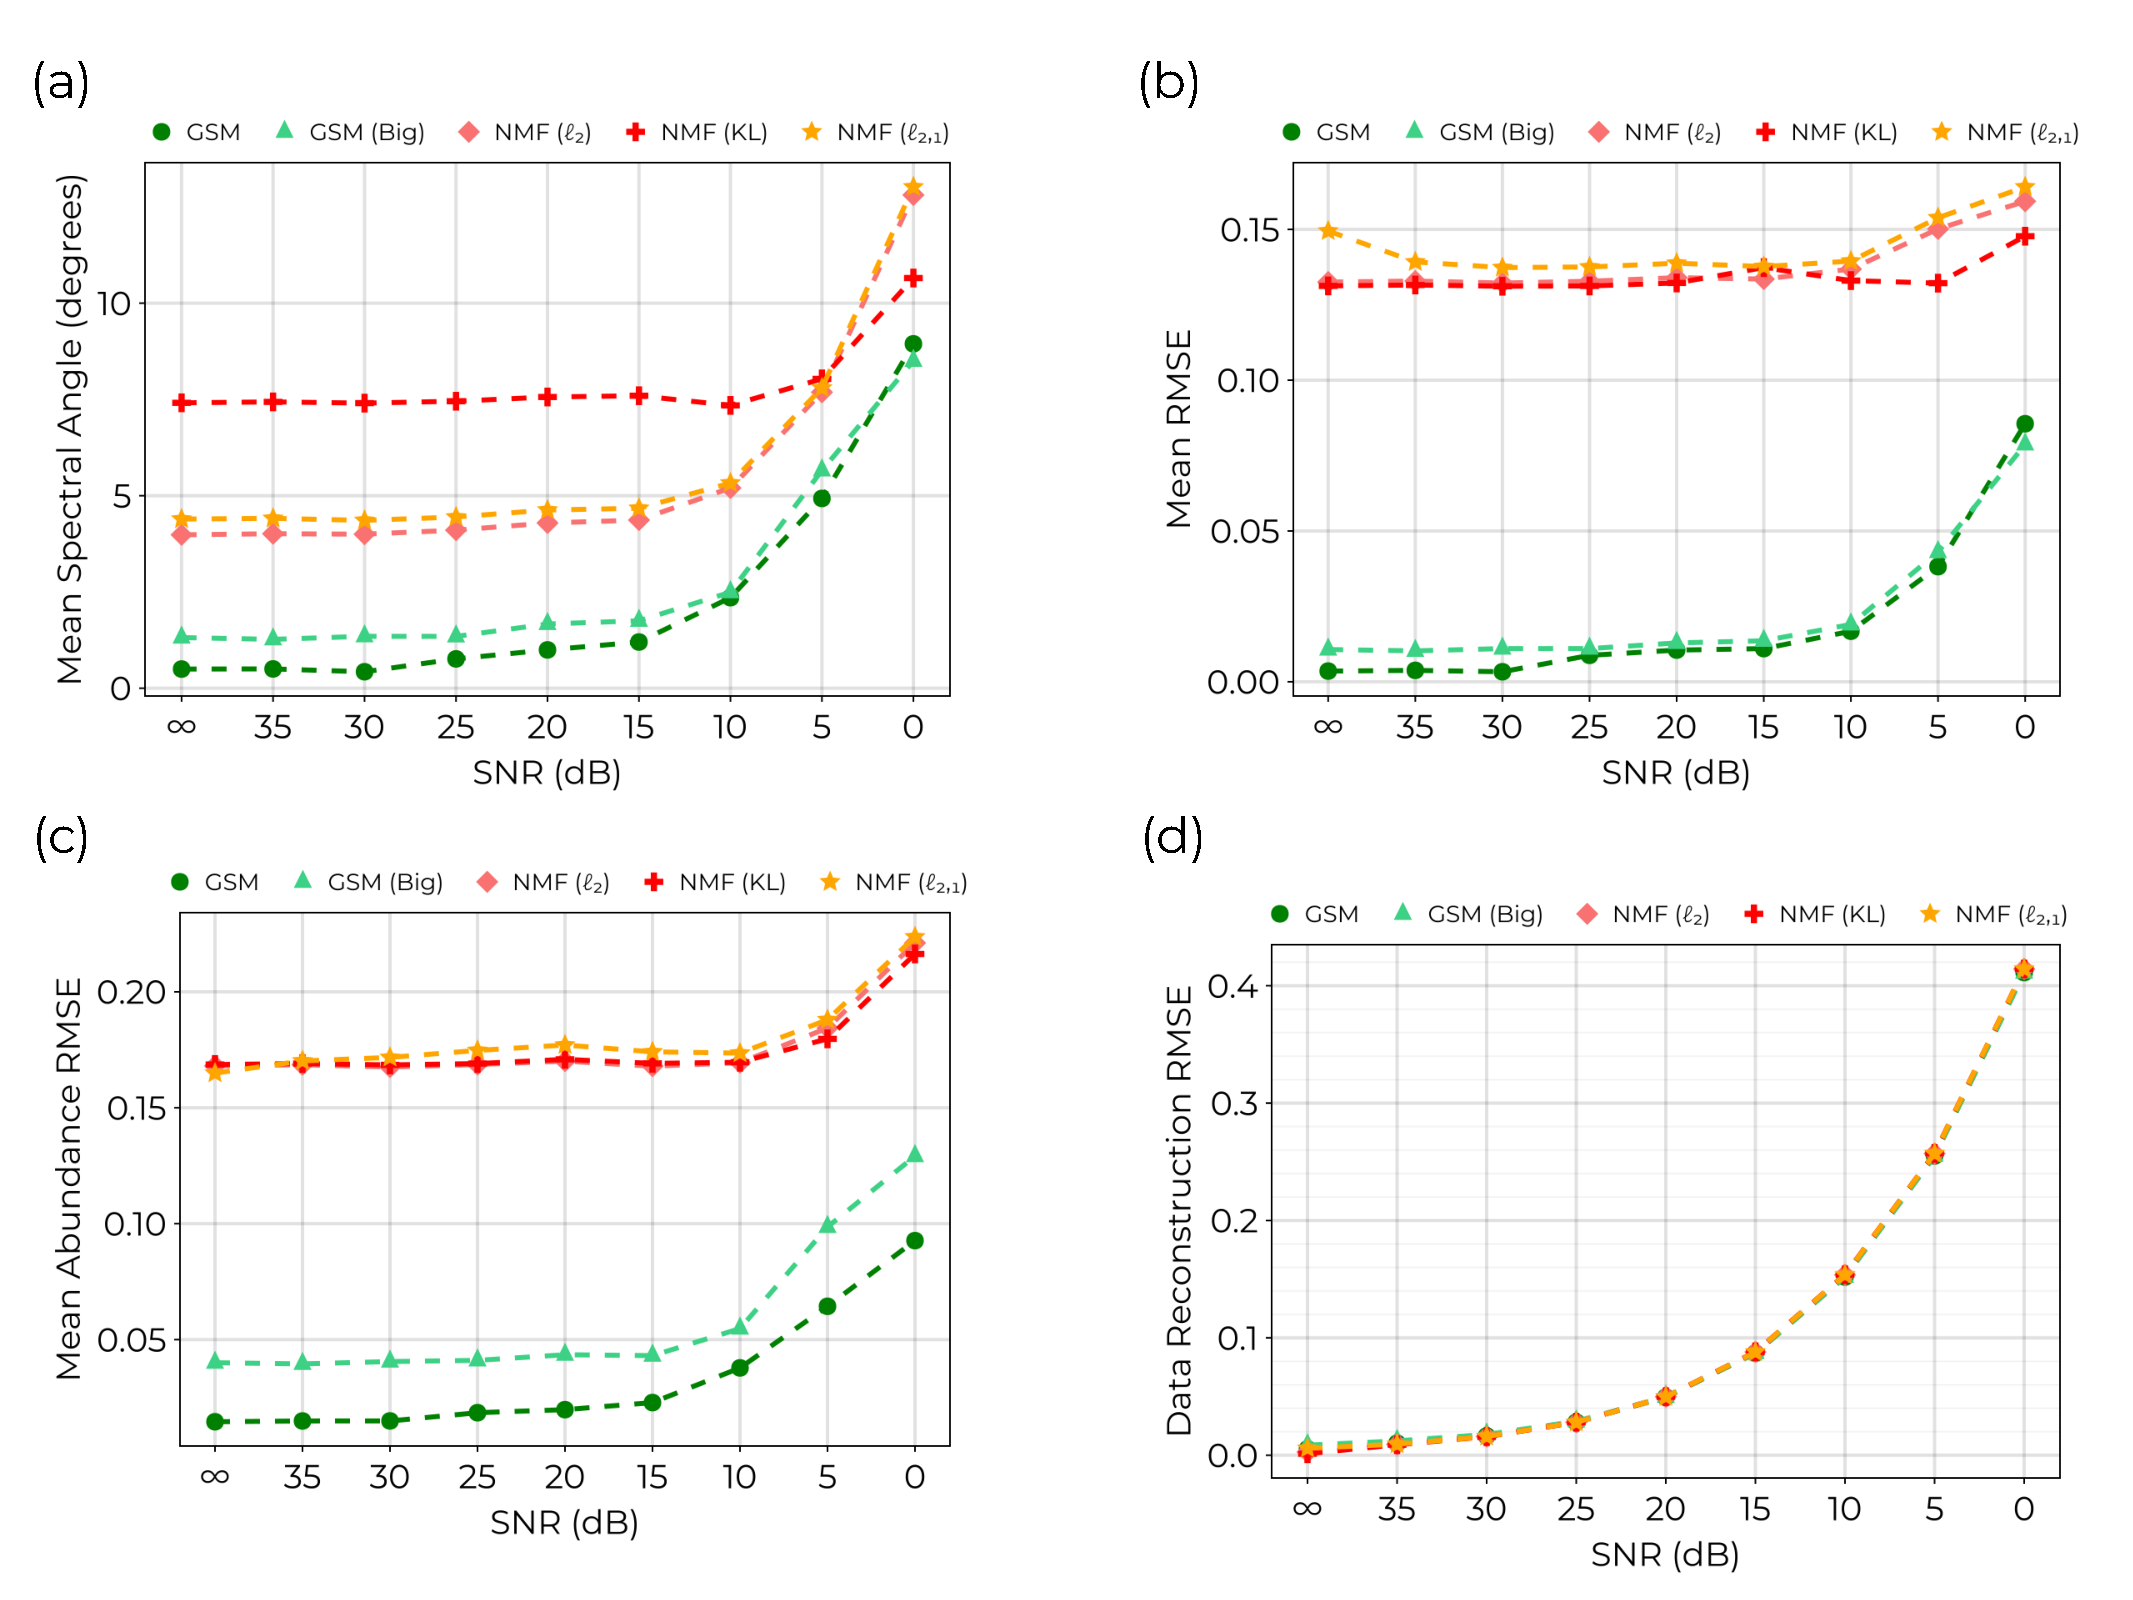
\includegraphics[width=\columnwidth]{robot-team-gsm/results/usgs/fit-comparison.pdf}
  \caption{Comparison of GSM against NMF on simulated linear mixing data set
    using USGS spectra. \textbf{(a)} The mean spectral angle computed between
    extracted endmembers and original endmembers. \textbf{(b)} the mean RMSE
    computed between extracted endmembers and original endmembers. \textbf{(c)}
    The mean abundance RMSE computed between original abundance data for each
    endmember and extracted abundances. \textbf{(d)} The reconstruction RMSE
    which evaluates the quality of fit. All models realized similar values
    reflecting convergence of the models to the level of random noise introduced
    into the data.}
  \label{fig:usgs-fits}
\end{figure}

The quality of endmember extraction is measured by the mean spectral angle and
the mean endmember RMSE. As Figure~\ref{fig:usgs-fits} indicates, both versions
of the GSM outperformed their NMF counterparts. Additionally, we note that for
all GSM models, even including $\text{SNR}=0$, all model weights $W_{dm}$ for
$m>N_v$ corresponding to non-linear mixing were driven identically to $0.0$.
This confirms that, for data sets with purely linear mixing and random noise,
the GSM correctly fits a mixing model without introducing unnecessary
complexity.

The quality of the unmixing, that is, the estimation of the abundance, performed
by each model was evaluated using the mean abundance RMSE. Here we again see
that both versions of the GSM outperformed NMF. To justify that all models were
fairly trained to convergence, the RMSE data reconstruction was also computed.
This metric uses the trained mixing model to compute the error between the
original data set and the reconstructed spectra generated using the extracted
endmembers and their abundances. For all GSM and NMF models, the RMSE data
reconstruction converged to the level of random noise introduced into the data.
These results reflect a fair comparison between the NMF and GSM models.

In Figure~\ref{fig:usgs-endmembers}, we plot the endmembers extracted for the
GSM model trained on the synthetic data set with $\text{SNR}=20$.

\begin{figure}[H]
  \centering
  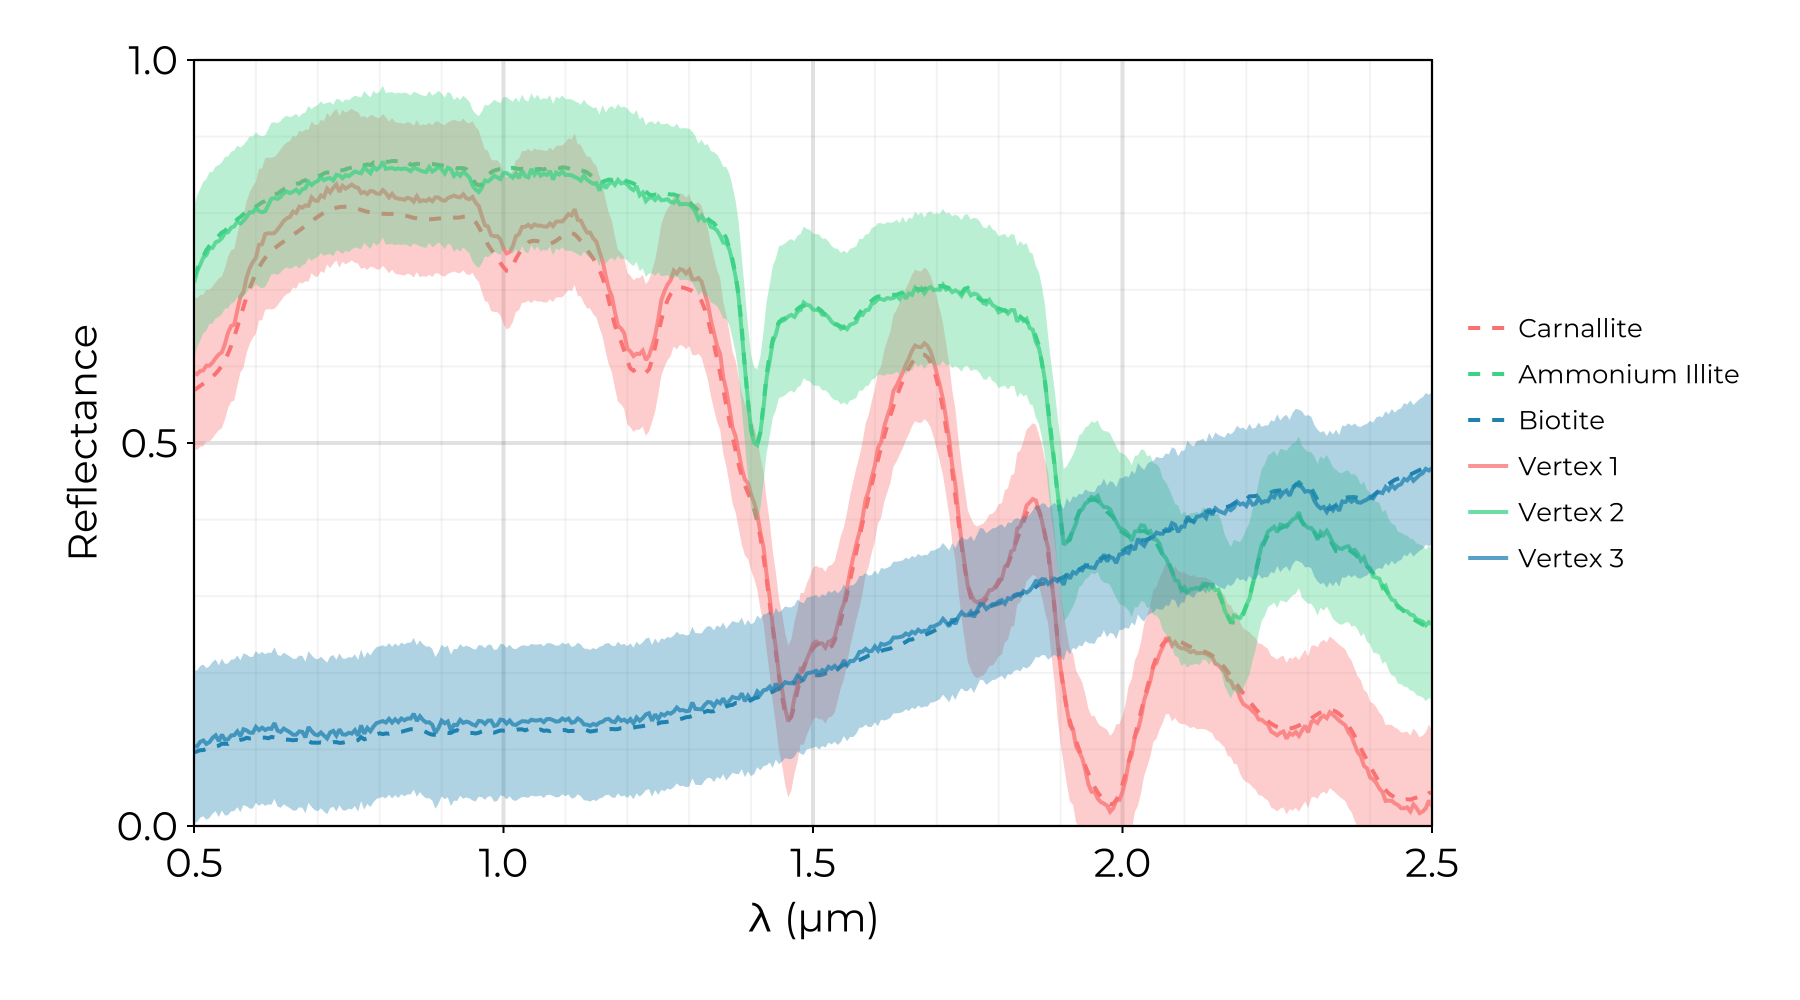
\includegraphics[width=\columnwidth]{robot-team-gsm/results/usgs/extracted-endmembers.png}
  \caption{Endmembers extracted by the GSM for the simulated linear mixing data
    set with SNR$=20$. The dashed lines correspond to original endmember spectra
    from the USGS spectral database. Solid lines superimposed on the plot
    indicate the extracted endmember spectra. Colored bands are included around
    each spectrum corresponding to the spectral variability estimated by the GSM
    precision parameter $\beta$ where the band width is $2\sqrt{\beta^{-1}}$
    corresponding to $2$ standard deviations.}
  \label{fig:usgs-endmembers}
\end{figure}

The extracted endmembers clearly fit the original source spectra while capturing
local reflectance features. Furthermore, the GSM precision parameter $\beta$
which is tuned during model training, provides an assessment of spectral
variability due to random noise. In Figure~\ref{fig:usgs-endmembers} this is
indicated by the colored band centered around each extracted spectrum with a
width of $2\sqrt{\beta^{-1}}$ corresponding to 2 standard deviations. The SNR of
$20$ added to this example corresponds to zero-mean Gaussian noise with a
standard deviation of $\sigma=0.0493$. After training, the GSM found
$\sqrt{\beta^{-1}}=0.0495$ that accurately captures the introduced noise. This
ability to assess the spectral variability of extracted endmembers is a key
advantage of the GSM.


\subsection{Non-linear Mixing: Rhodamine Dye Plume}

For the data set of real HSI spectra described in Section~\ref{sec:real-experiments},
80 GSM models were trained to explore the GSM hyperparameter space. The
performance of the model was compared using the BIC, AIC and RMSE reconstruction
with the results of the top $10$ performing models shown in
Table~\ref{table:fit-comparison}.

\begin{table}[H]
  \caption{GSM hyperparameter optimization for the real HSI data set: Multiple
    GSM models were trained to explore the impact of model hyperparameters.
    $N_v$ values from $3$ to $6$ were explored as suggested by the PCA
    decomposition of the data set. $\lambda_e$ was varied from $0.001$ to $1.0$
    and $\lambda_w$ ranged from $1$ to $1000$. Here we report the top $10$
    models ranked by increasing BIC. The AIC and reconstruction RMSE are also
    included for comparison.}
  \label{table:fit-comparison}
  \begin{center}
  \begin{tabular}{cccccc} \hline
    \textbf{$N_v$}	& \textbf{$\lambda_e$}	& \textbf{$\lambda_w$} &
    \textbf{BIC} & \textbf{AIC} & \textbf{Reconstruction RMSE}\\ \hline
    $3$ & $0.01$    & $1.0$     & $-6.195\times10^7$   & $-6.269\times10^7$   & $0.000989$ \\
    $3$	& $0.001$   & $1.0$     & $-6.194\times10^7$   & $-6.268\times10^7$   & $0.000989$ \\
    $3$	& $0.1$     & $1.0$	    & $-6.192\times10^7$   & $-6.265\times10^7$   & $0.000991$ \\
    $3$	& $1.0$     & $1.0$	    & $-6.186\times10^7$   & $-6.260\times10^7$   & $0.001190$ \\
    $4$	& $1.0$     & $1.0$	    & $-6.181\times10^7$   & $-6.255\times10^7$   & $0.001002$ \\
    $4$	& $0.1$     & $1.0$	    & $-6.175\times10^7$   & $-6.249\times10^7$   & $0.001008$ \\
    $4$	& $0.01$    & $1.0$     & $-6.173\times10^7$   & $-6.247\times10^7$   & $0.001009$ \\
    $4$	& $0.001$   & $1.0$     & $-6.173\times10^7$   & $-6.247\times10^7$   & $0.001009$ \\
    $4$	& $0.1$     & $10.0$    & $-6.171\times10^7$   & $-6.245\times10^7$   & $0.001011$ \\
    $3$	& $1.0$     & $10.0$    & $-6.166\times10^7$   & $-6.239\times10^7$   & $0.001014$
  \end{tabular}
  \end{center}
\end{table}

As the table indicates, a non-linear GSM with $N_v=3$, $\lambda_e=0.01$, and
$\lambda_w=1.0$ achieved minimum BIC, AIC, and reconstruction RMSE values. The
lower value of $\lambda_w$ identified from these models reflects the presence of
non-linear mixing effects in the HSI data. Although the values of model weights
$W_{dm}$ for $m>N_v$ corresponding to non-linear mixing were $0$ for the
synthetic data set, here these weights obtained a small but non-negligible
median value of $0.0012$.


Reflectance spectra generated by the trained GSM corresponding to the maximum
abundance values for each endmember are plotted in
Figure~\ref{fig:robot-team-endmembers}. Based on their signatures, these
endmembers are identified with water, vegetation (including near shore,
filamentous blue-green algae) and the rhodmaine dye plume.

\begin{figure}[H]
  \centering
  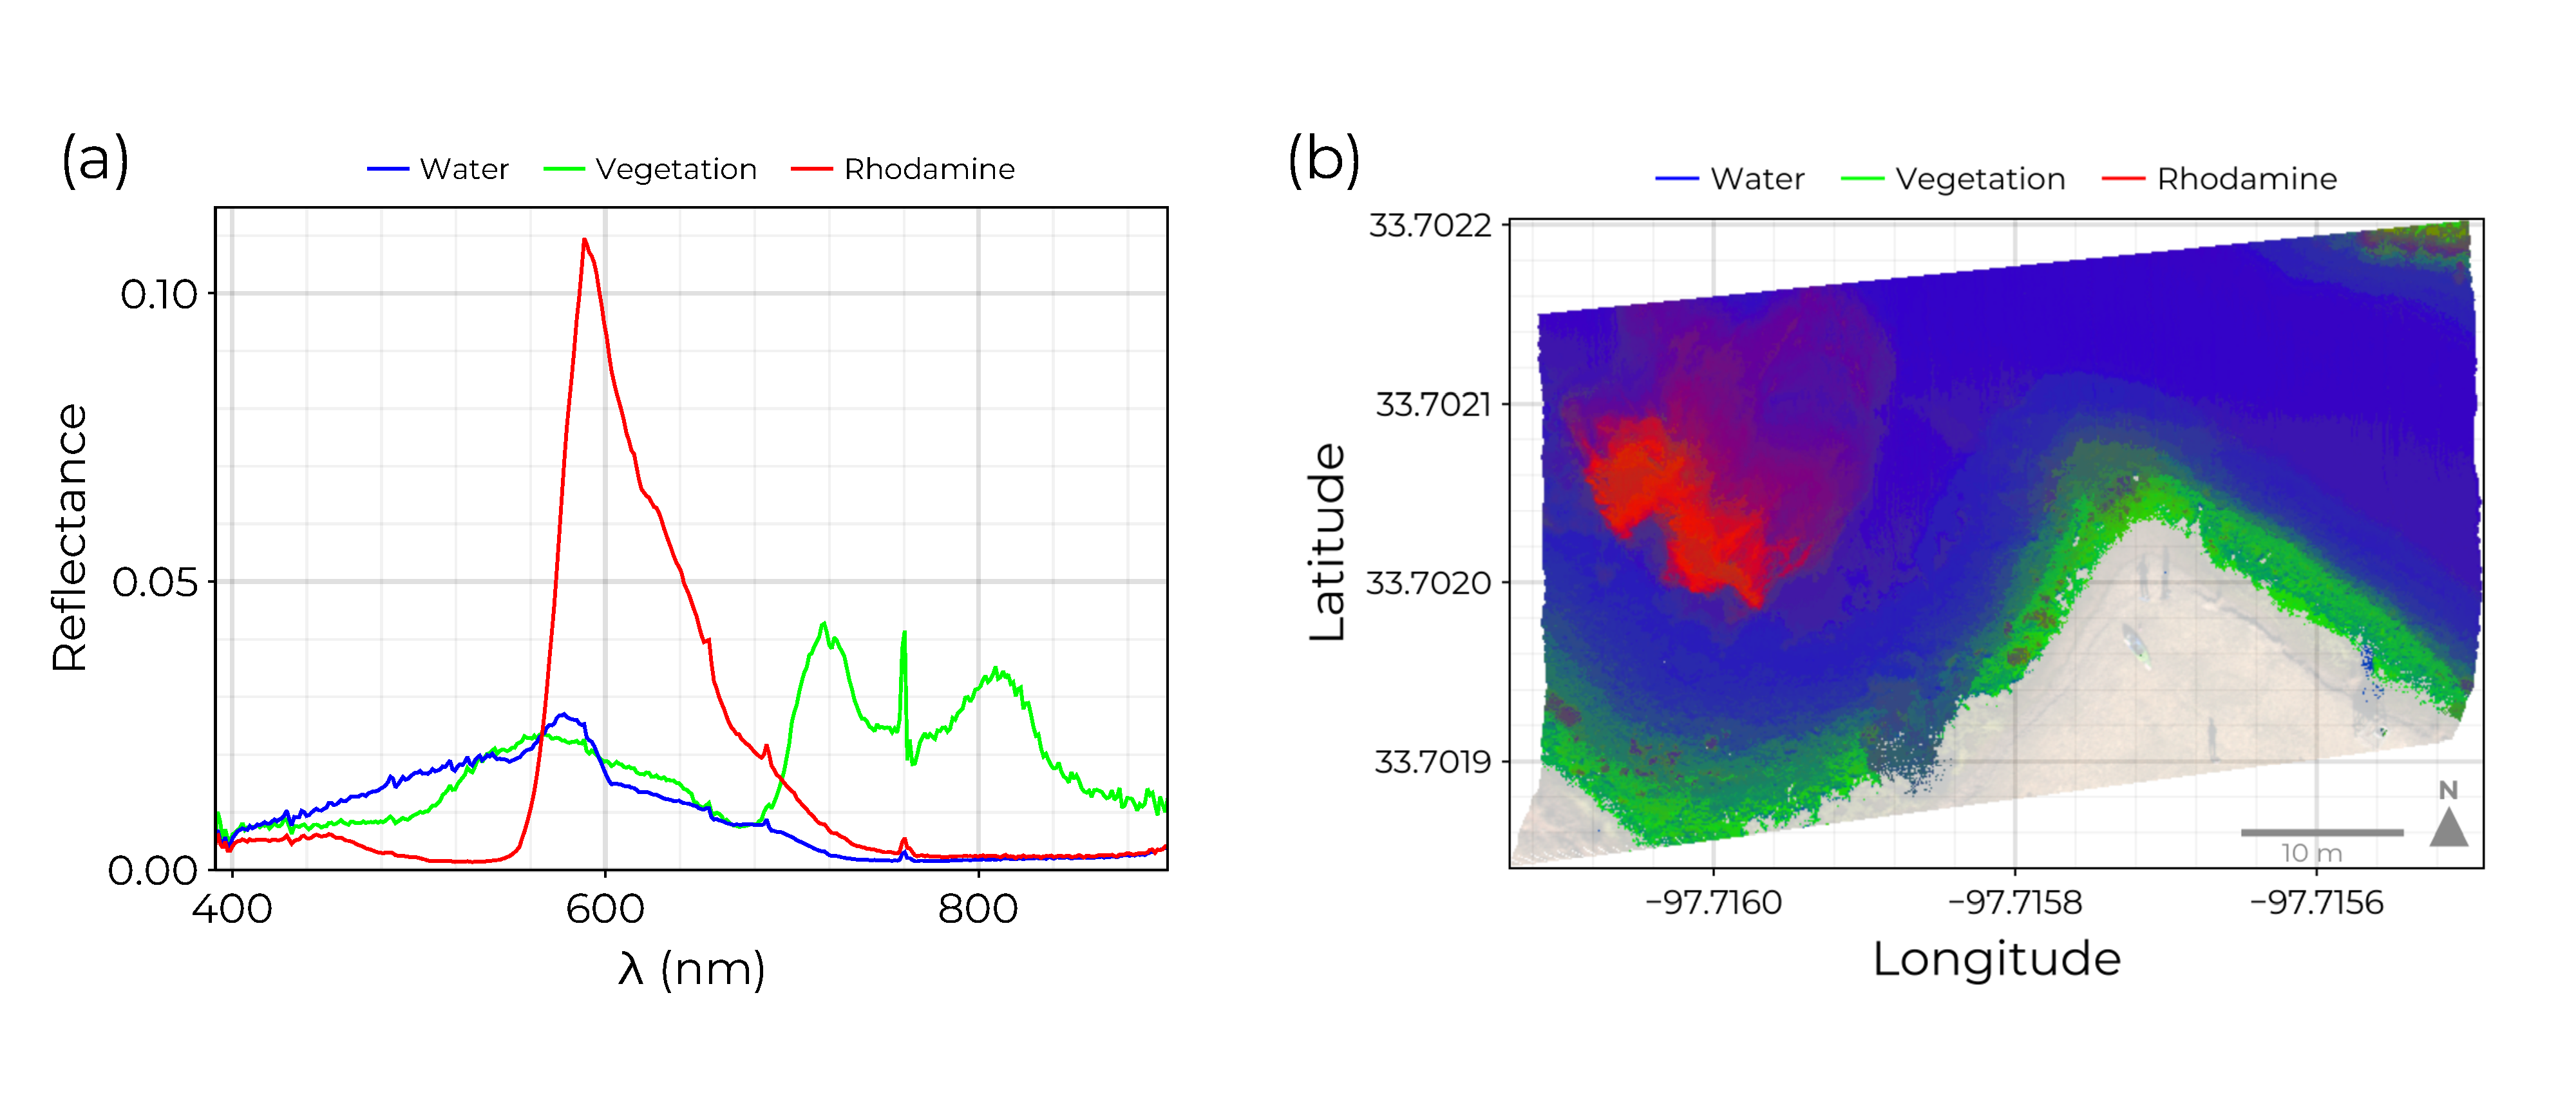
\includegraphics[width=\columnwidth]{robot-team-gsm/results/robot-team/extracted-endmembers.pdf}
  \caption{GSM applied to water spectra from real HSI data set: \textbf{(a)}
    Spectra generated by the trained GSM for samples with maximum abundance for
    each endmember. Based on these spectral profiles, endmembers are identified
    with water, near-shore vegetation, and rhodamine dye. \textbf{(b)} A HSI
    segmented according to the relative abundance of each endmember. Each water
    pixel is colored by smoothing interpolating between red, green, and blue
    colors using the relative abundance estimated for rhodamine, vegetation, and
    water spectra. The rhodamine plume is clearly identifiable in the western
    portion of the HSI.}
  \label{fig:robot-team-endmembers}
\end{figure}



% \clearpage
% \newpage

% \begin{sidewaysfigure}
%   \centering
%   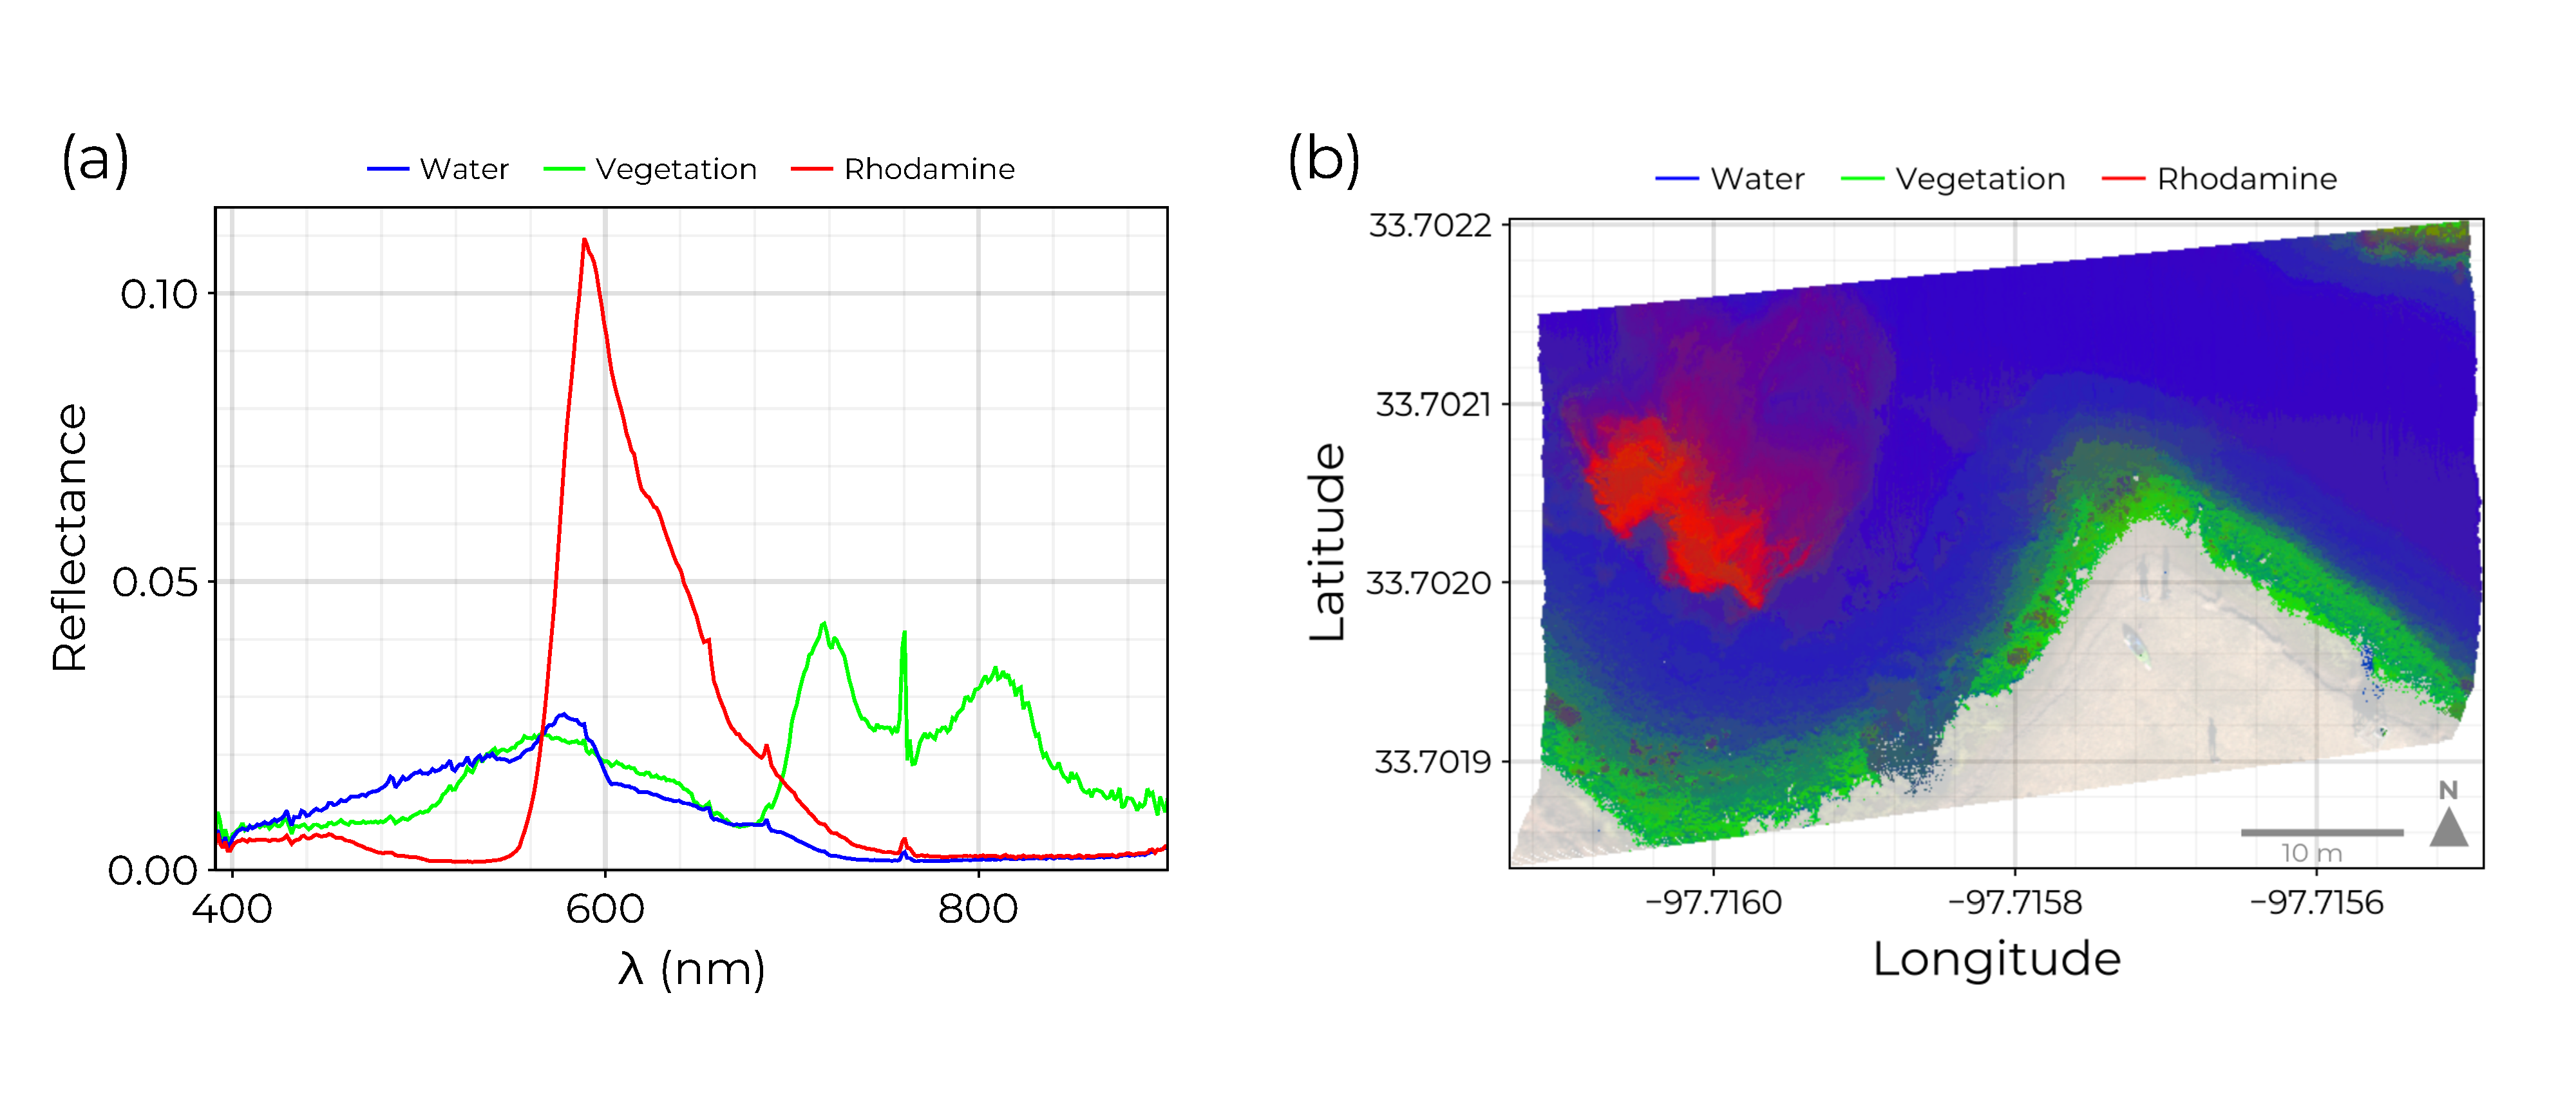
\includegraphics[width=\columnwidth]{robot-team-gsm/results/robot-team/extracted-endmembers.pdf}
%   \caption{GSM applied to water spectra from real HSI data set: \textbf{(a)}
%     Spectra generated by the trained GSM for samples with maximum abundance for
%     each endmember. Based on these spectral profiles, endmembers are identified
%     with water, near-shore vegetation, and rhodamine dye. \textbf{(b)} A HSI
%     segmented according to the relative abundance of each endmember. Each water
%     pixel is colored by smoothing interpolating between red, green, and blue
%     colors using the relative abundance estimated for rhodamine, vegetation, and
%     water spectra. The rhodamine plume is clearly identifiable in the western
%     portion of the HSI.}
%   \label{fig:robot-team-endmembers}
% \end{sidewaysfigure}

% \clearpage
% \newpage

By assigning a unique color to each endmember, the spatial distribution of HSI
spectra can be visualized by using estimated abundances to smoothly interpolate
between endmember colors as shown in panel b of
Figure~\ref{fig:robot-team-endmembers}. In other words, this method provides a
fuzzy semantic segmentation of HSI pixels. Alternatively, each HSI pixel could
be assigned a single class corresponding to the endmember with maximal
abundance. In this way, the GSM can be used to visualize high-dimensional HSI
spectra.


To showcase the ability of the GSM to identify spatially localized contaminant
sources, abundance maps were generated for each individual end member using the
trained GTM to unmix all water pixels in the HSI. In
Figure~\ref{fig:endmember-abundance-dist} these abundance maps are compared for
each endmember. The abundance map for the water endmember covers a majority of
the center of the pond and decreases near the edge of the rhodamine plume where
the dye and water mix. The vegetation in shallow water near the shore and the
rhodamine dye plume in the western half of the pond are also clearly identified
by their abundance maps. Given an HSI pixel resolution of $0.1 \times 0.1$
$\text{m}^2$, the spatial extent of vegetation is estimated to be $378.6$
$\text{m}^2$ while the plume initially extends across $255.7$ $\text{m}^2$.


\newpage

\begin{figure}[H]
  \vspace{-1.5cm}
  \centering
  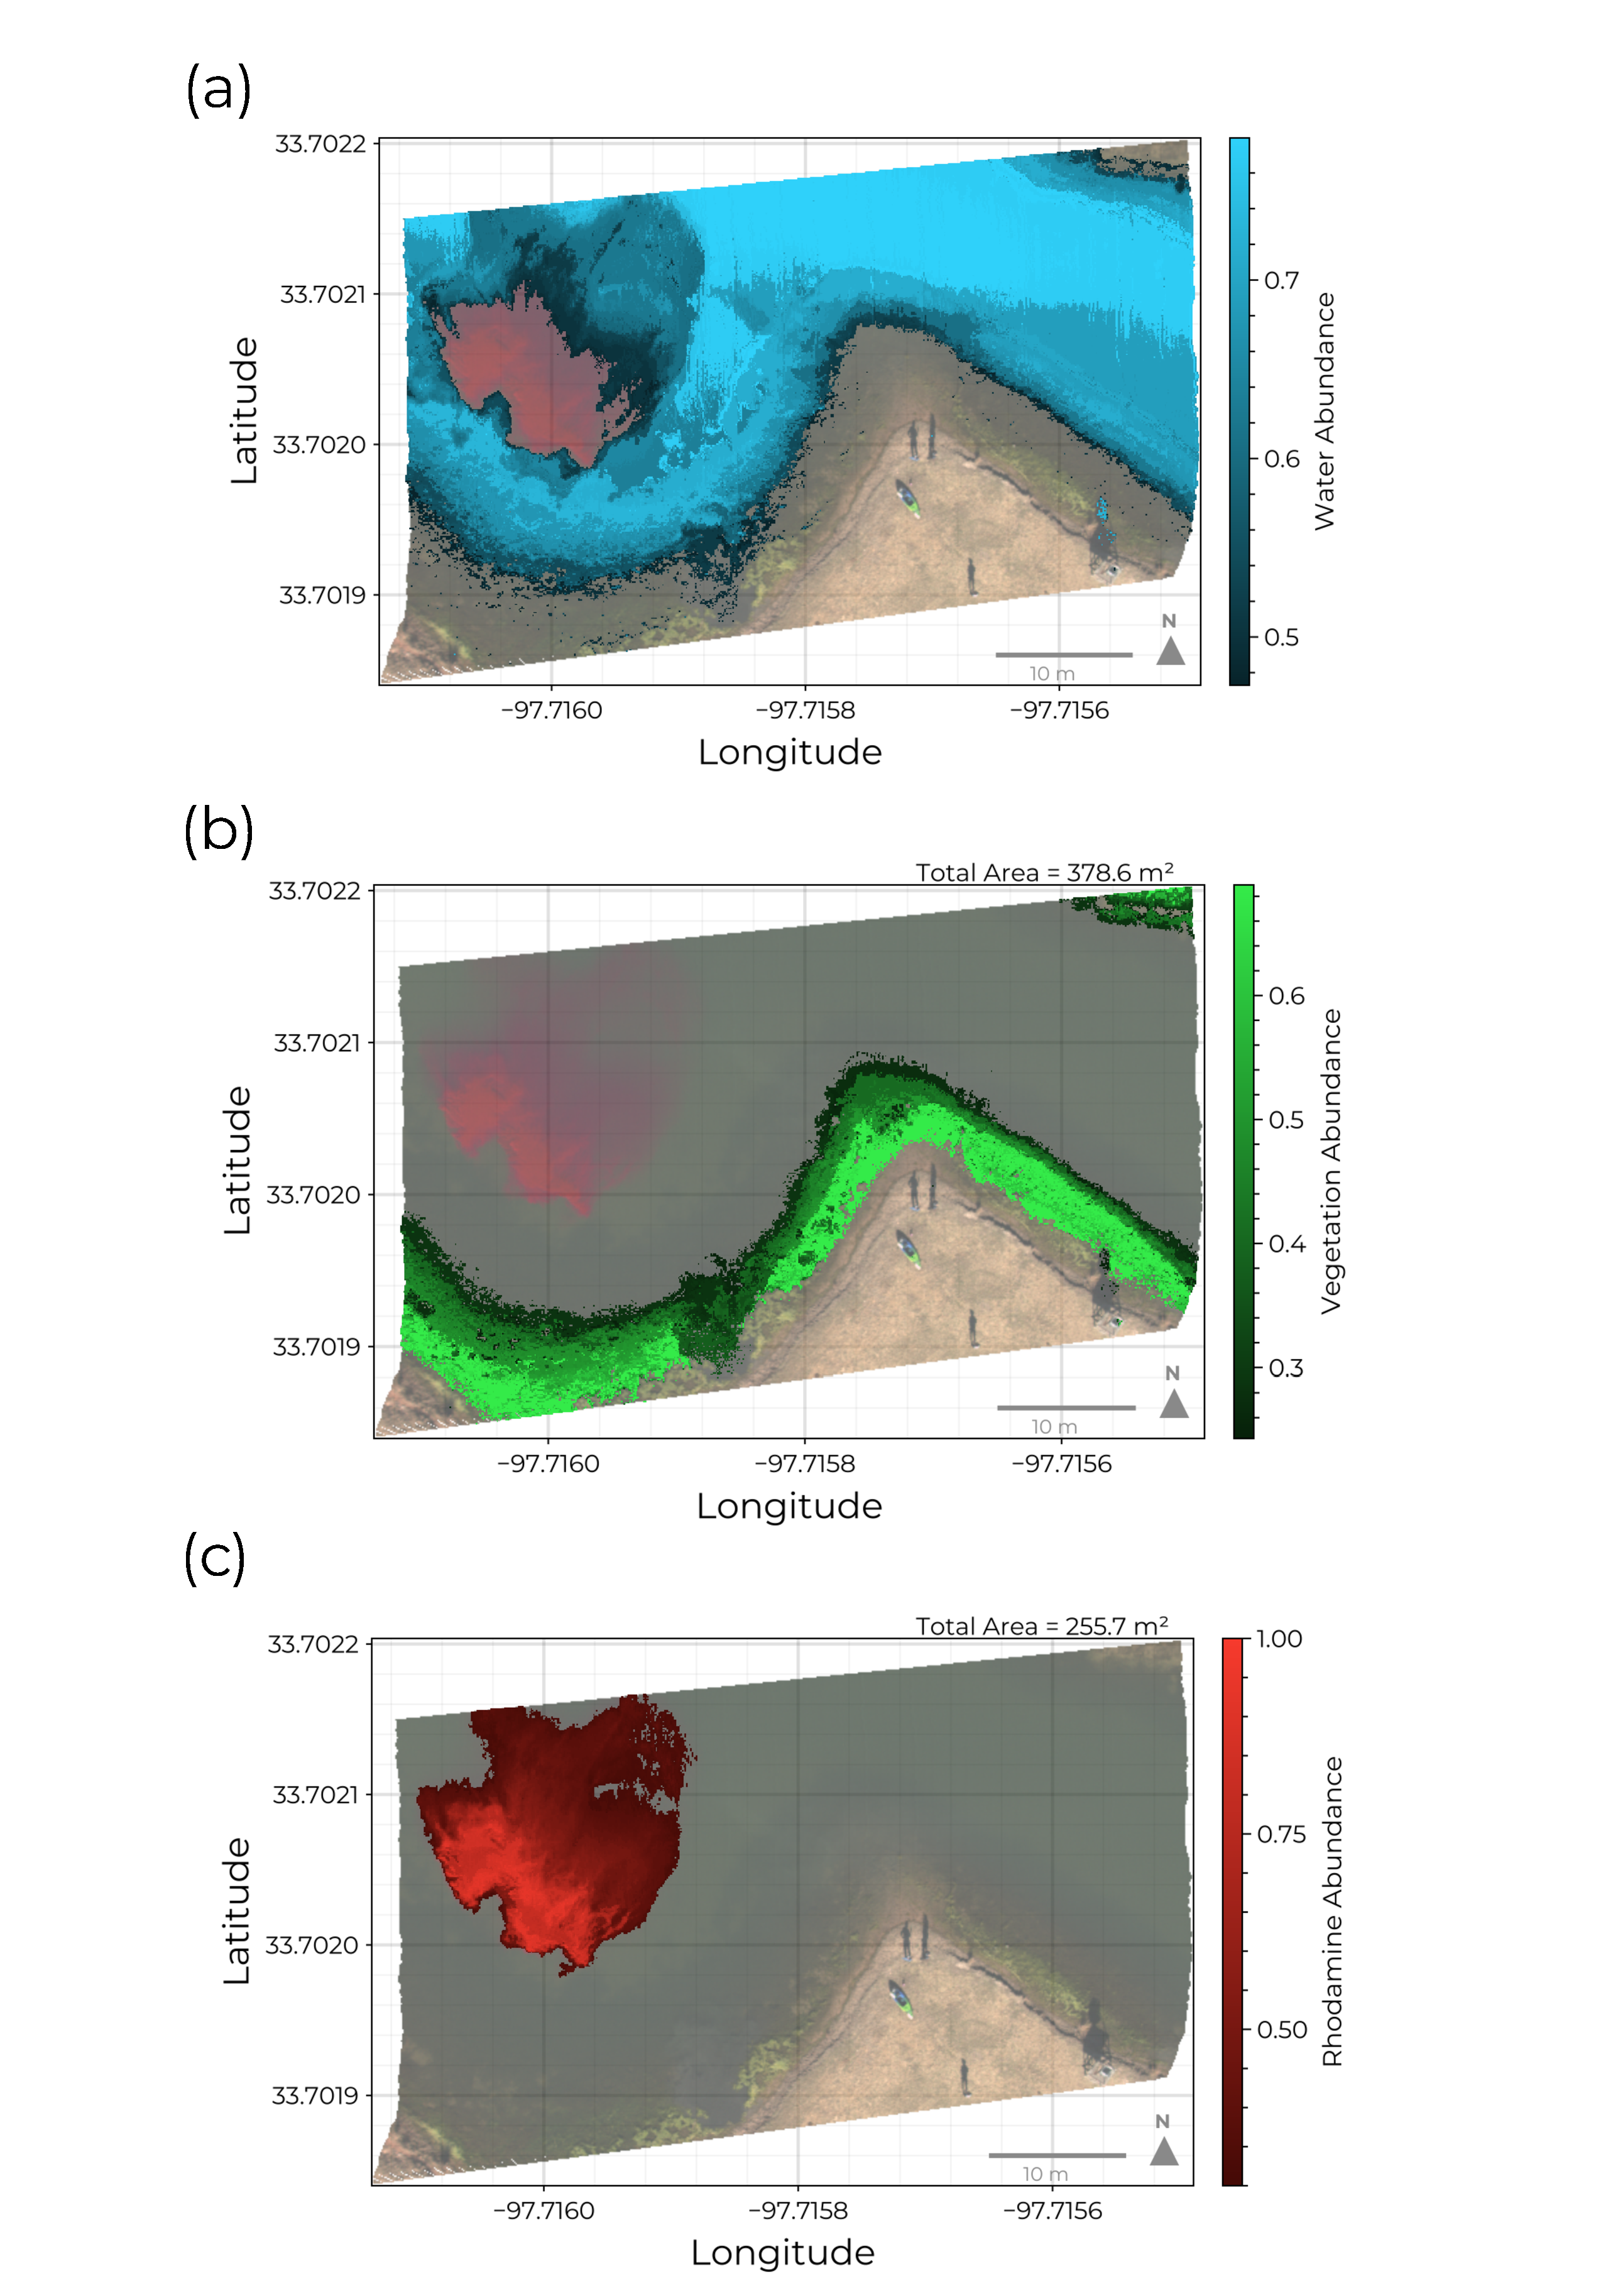
\includegraphics[width= 0.8\columnwidth]{robot-team-gsm/results/robot-team/endmember-abundances.pdf}
  \caption{Endmember abundance distributions: \textbf{(a)} The spatial
    distribution of abundance for the water class. This source dominates in the
    center of the pond and decreases towards the shore where vegetation begins
    to dominate the reflectance signal. The water endmember abundance is also
    observed to decreases near the edge of the rhodamine plume reflecting dye
    mixing and diffusion. \textbf{(b)} The spatial distribution of vegetation.
    This endmember includes filamentous blue-green algae observed to accumulate
    in shallow waters near the shore. \textbf{(c)} The rhodamine dye plume
    extent segmented from the HSI. The total area for near-shore vegetation and
    rhodamine are estimated to be $378.6$ $\text{m}^2$ and $255.7$ $\text{m}^2$,
    respectively.}
  \label{fig:endmember-abundance-dist}
\end{figure}


Applying the trained GSM to unmix HSI from UAV flights provides an efficient way
to map the dispersion and transport of contaminant. Figure~\ref{fig:plume-evo}
demonstrates this by mapping the growing extent of rhodamine dye between
successive UAV flights. In just $15$ minutes, the plume expands from an initial
area of $255.7$ $\text{m}^2$ to over $571.8$ $\text{m}^2$ as the dye mixes with
the surrounding water.


\clearpage
\newpage

\begin{sidewaysfigure}
  \centering
  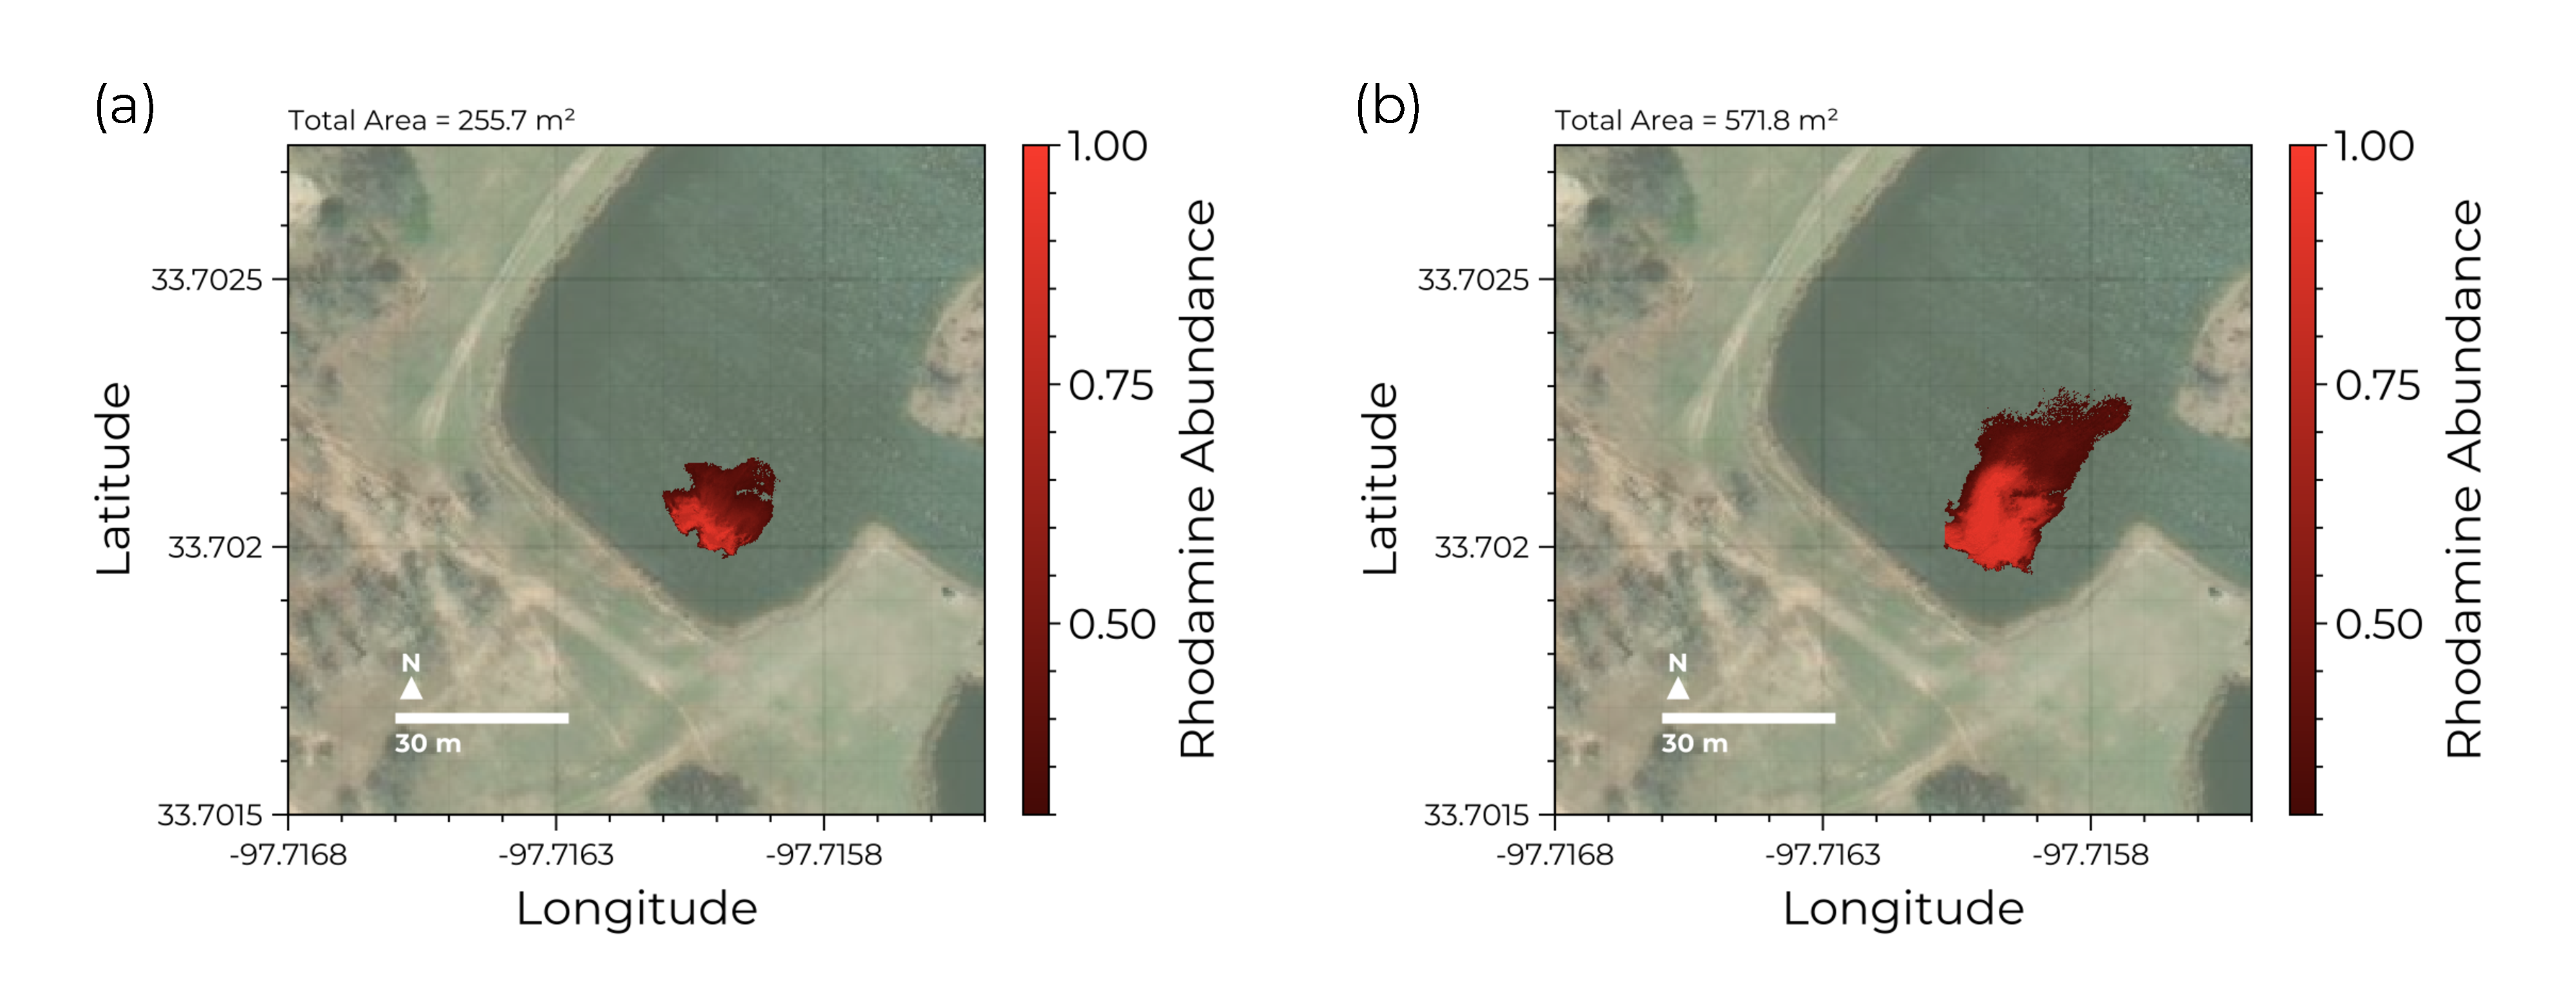
\includegraphics[width=\columnwidth]{robot-team-gsm/results/robot-team/plume-evo.pdf}
  \caption{Rhodamine plume evolution: Using the trained GSM we can track the
    dispersion of the rhodamine dye plume between successive drone flights.
    \textbf{(a)} The initial plume distribution after release. Here the dye
    subsumes an area of $255.7$ $\text{m}^2$. \textbf{(b)} The same plume imaged
    15 minutes later now extends across an area of $571.8$ $\text{m}^2$}
  \label{fig:plume-evo}
\end{sidewaysfigure}



% \begin{figure}[H]
%   \centering
%   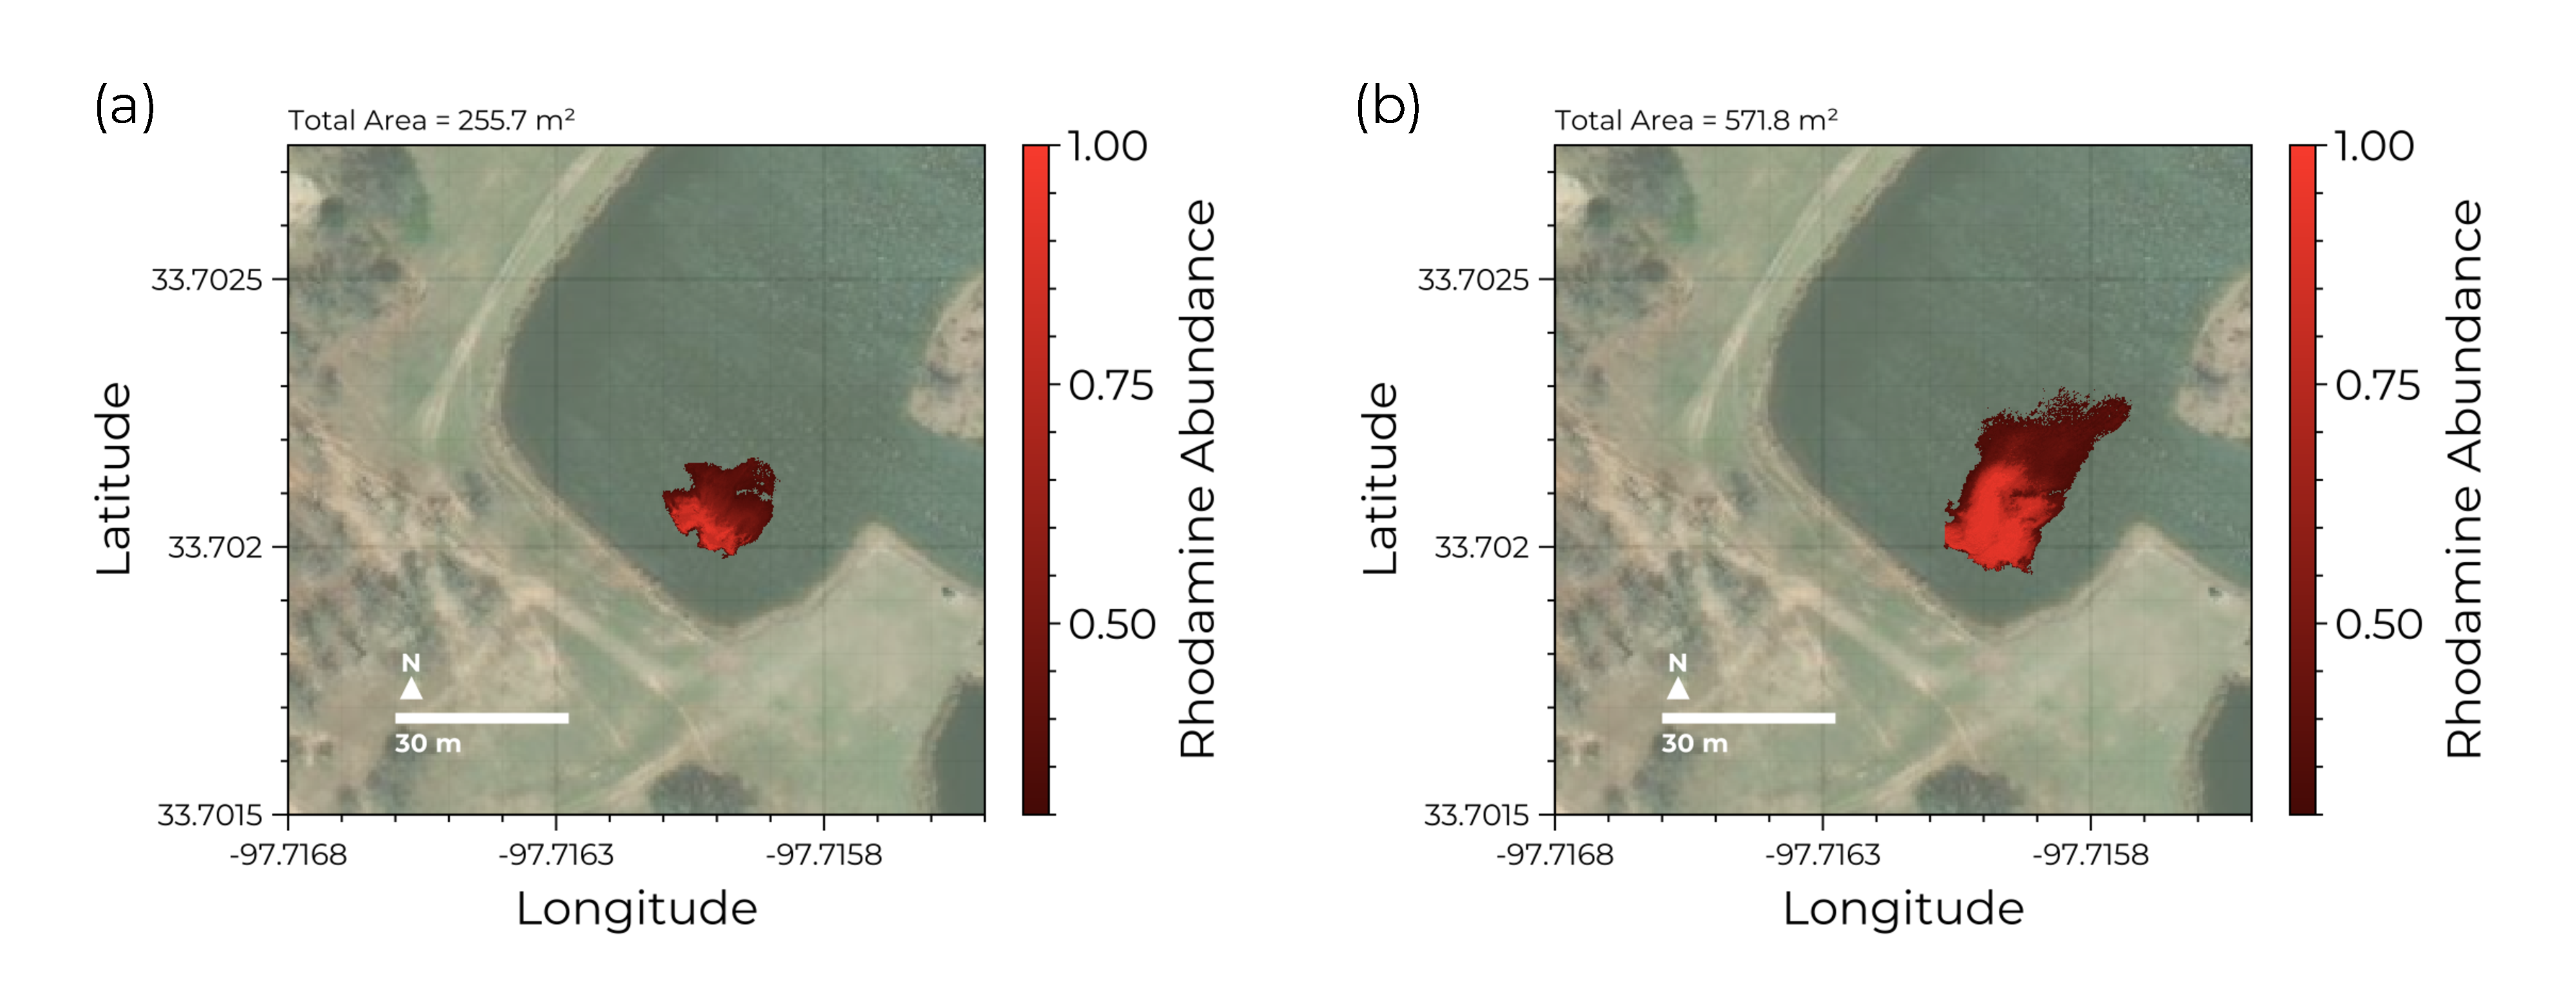
\includegraphics[width=\columnwidth]{robot-team-gsm/results/robot-team/plume-evo.pdf}
%   \caption{Rhodamine plume evolution: Using the trained GSM we can track the
%     dispersion of the rhodamine dye plume between successive drone flights.
%     \textbf{(a)} The initial plume distribution after release. Here the dye
%     subsumes an area of $255.7$ $\text{m}^2$. \textbf{(b)} The same plume imaged
%     15 minutes later now extends across an area of $571.8$ $\text{m}^2$}
%   \label{fig:plume-evo}
% \end{figure}


\clearpage
\newpage

\section{Discussion}


The proliferation of hyperspectral imaging technologies in the remote sensing
and environmental monitoring communities underscores the need for efficient
algorithms that can make sense of high-dimensional HSI. Of particular interest
are unsupervised algorithms which utilize all available wavelength bins to
identify unique source profiles that present realistic scenes. The GSM
introduced in this study is a novel method that simultaneously performs
endmember extraction and spectral unmixing. Unlike popular endmember extraction
algorithms, such as VCA, PPI, and N-FINDR, GSM does not assume the presence of
pure pixels in HSI. Furthermore, the flexible structure of the mapping from the
GSM latent space to the spectral data space allows the GSM to model non-linear
mixing effects, distinguishing it from other widely used linear models such as
NMF. Being a probabilistic model also enables the GSM to quantify the spectral
variability through the precision parameter $\beta$ as indicated in
Figure~\ref{fig:usgs-endmembers}. This additional capability is critical for
analysis of realistic HSI where sensor noise, viewing geometry, and scene
illumination all introduce uncertainty into extracted endmembers.


The growing popularity of deep learning methods has led many to explore
applications of deep learning to the spectral unmixing problem. Variations in
auto-encoder architectures are a popular choice for both endmember extraction
and unmixing. For example, Borsoi et al. used a variational autoencoder to more
accurately identify the spectral variability in a LMM \cite{borsoi2019deep}.
Similarly, Palson et al. introduced an autoencoder with convolution layers to
extend the LMM by incorporating spatial context from neighboring HSI pixels
\cite{palsson2020convolutional}. However, the increased complexity of deep
neural network approaches makes interpreting the latent space learned by encoder
layers challenging and can dramatically increase training time and data volume
requirements. In contrast, the latent space of the GSM is immediately
interpretable due to the imposed simplex geometry, while the form of $\psi$
leaves room to explore a variety of non-linear mixing models. In this study,
$\psi$ was constructed to add non-linear effects as additions or perturbations
to an underlying linear mixing model with the $\lambda_w$ hyperparameter
provided to control the degree of non-linearity considered. In the original GTM
formulation that inspired the GSM, the mapping $\psi$ strictly uses non-linear
features generated by Gaussian RBFs. Alternatively, one could easily construct
$\psi$ for specific non-linear models such as bilinear mixing by introducing
features which depend on higher-order combinations of the latent space
(abundance) coordinates. However, it is important to note that the EM algorithm
formulated for GSM training is made possible due to the linear combination of
activations $\phi(\mathbf{z})$ with model weights $\mathbf{W}$. For mixing
models which instead depend non-linearly on weights $\mathbf{W}$, an EM
algorithm may require iterative non-linear solves during each M step.


The main limitation of the GSM is the curse of dimensionality encountered when
generating a grid on the $(N_v-1)$-simplex for large numbers of endmembers,
$N_v$. This can be mitigated by instead randomly sampling points within the
interior of the simplex using a uniform Dirichlet distribution to obtain a
pre-determined number of nodes across the latent space. As the mixing
coefficients $\pi_k$ are adapted during training, the variability in the spacing
of the internodes should not significantly affect the performance of the model.
In fact, this was confirmed for the simulated data set as summarized in
Figure~\ref{fig:usgs-fits}. For considerably large data sets, the size of the
responsibility matrix $\mathbf{R}$ can also lead to extended training times.
This can be addressed by augmenting the EM procedure to updated using
mini-batches of training samples during each E-step as described by Bishop et
al. for the GTM in ref. \cite{gtm-developments}. Rather than updating the full
responsibility matrix, a subset of $\mathbf{R}$ corresponding to a single batch
of training data can be evaluated with all other entries kept constant. The GSM
may also be extended in other ways, for example, by replacing the precision
parameter $\beta$ with a covariance matrix to model wavelength-dependent
spectral variability common to many hyperspectral imaging platforms.


Based on the results of applying the GSM to real HSI as illustrated in
Figure~\ref{fig:endmember-abundance-dist} and Figure~\ref{fig:plume-evo}, one
clear application of the GSM is to contaminant identification and water quality
assessment. Modern UAV platforms make it possible to rapidly image bodies of
water where direct access for in-situ data collection is restricted. By
equipping UAVs with hyperspectral imagers, the GSM can be used to identify
abnormal spectral signatures corresponding to localized contaminant sources.
Generating semantic segmentations of collected HSI as in panel b of
Figure~\ref{fig:robot-team-endmembers} makes it easy to compare multiple HSI
without resorting to pseudocolor images generated from a limited number of
wavelength bands. Since the GSM models the distribution of all HSI spectra
rather than individual parameters, it may also aid in-situ data collection by
suggesting sampling points which maximize the area traversed in the GSM latent
space rather than uniformly sampling across a wide spatial extent. Similar
approaches have been developed to guide autonomous data collection vehicles by
casting route planning as a prize collecting travelling salesman problem subject
to resource constraints \cite{balas2007prize, suryan2020learning}.


As a final consideration, we note that the problem of endmember extraction and
spectral unmixing for HSI is identical to source apportionment in the context of
air quality. Here, the goal is to identify measurement profiles associated with
sources of ambient air pollution based on measurements at a receptor site. A
popular model for source apportionment studies is Positive Matrix Factorization
(PMF) introduced by Paatero and Tapper \cite{pmf-orig,
  ulbrich2009interpretation}. Just like NMF, PMF decomposes measurements into a
linear combination of source profiles and relative abundances subject to
non-negativity constraints. These linear receptor models assume that the sources
are not transformed during transport to the receptor, ignoring changes due to
chemical reactions. Non-linear mixing models such as the GSM introduced here
may, therefore, prove beneficial in this additional domain.


